%\nocite{a565d200}
%\nocite{69cbf29c}
%TODO
%  improve $2$-category definitions (weak and strict) with better notation and more terminology
We now turn to a somewhat more sophisticated construction involving categories completing the holy trinity of category theory. Namely natural transformations. Loosely speaking, this is a transformation between two functors obtained from an observation in algebraic topology. A set $\mathsf{T}$ is a \textbf{natural transformation} (abbr.: nat. trans.) or \textbf{natural} if it is a $3$-tuple consisting of a functor $F$, a functor $F^{\backprime}$ such that
\begin{align*}
  \mathrm{dom_{F}}(F)
  &=
  \mathrm{dom_{F}}(F^{\backprime})
  \\
  \mathrm{cod_{F}}(F)
  &=
  \mathrm{cod_{F}}(F^{\backprime})
\end{align*}
and a function
\begin{align*}
  \tau
  \colon
  \mathrm{ob}_{\mathrm{dom_{F}}(F)}
  &\rightarrow
  \mathrm{Mor}_{\mathrm{cod_{F}}(F)}
\end{align*}
that assigns to each object $X \in \mathrm{ob}_{\mathrm{dom_{F}}(F)}$ a morphism
\begin{align*}
  \tau(X)
  &\in
  \mathrm{mor}_{\mathrm{cod_{F}}(F)}(F(X),F^{\backprime}(X))
\end{align*}
such that
\begin{enumerate}
\item[(NT)]
for all $X_{1},X_{2} \in \mathrm{ob}_{\mathrm{dom_{F}}(F)}$ and $f_{12} \in \mathrm{mor}_{\mathrm{dom_{F}}(F)}(X_{1},X_{2})$ the equality
\begin{align*}
  F^{\backprime}(f_{12})
  \circ
  \tau(X_{1})
  &=
  \tau(X_{2})
  \circ
  F(f_{12})
\end{align*}
holds
\end{enumerate}
The naturality property (NT) is illustrated by a commutative diagram
\[
\begin{tikzcd}[sep=large]
  F(X_{1})
  \arrow{r}{F(f_{12})}
  \arrow[swap]{d}{\tau(X_{1})}
  &
  F(X_{2})
  \arrow{d}{\tau(X_{2})}
  \\
  F^{\backprime}(X_{1})
  \arrow{r}{F^{\backprime}(f_{12})}
  &
  F^{\backprime}(X_{2})
\end{tikzcd}
\]
Instead of {\glqq}a natural transformation $\mathsf{T} := (F,F^{\backprime},\tau)${\grqq} we write {\glqq}a natural transformation $\mathsf{T} \colon F \Rightarrow F^{\backprime}${\grqq}. Don't mix up this $\Rightarrow$ with the logical connective of implication - at least not without UFP-HoTT. It should rather indicate that a natural transformation is a $2$-arrow. For a natural transformation $\mathsf{T} \colon F \Rightarrow F^{\backprime}$ we call $F$ the \textbf{domain (of $\mathsf{T}$)} and $F^{\backprime}$ the \textbf{codomain (of $\mathsf{T}$)}. This defines assignments $\mathrm{dom_{T}}$ and $\mathrm{cod_{T}}$ assigning to a natural transformation its domain and codmain, respectively. $\mathrm{dom_{T}}$ is called \textbf{(nat. trans.) domain (assignment)} and $\mathrm{cod_{f}}$ is called \textbf{(nat. trans.) codomain (assignment)}. A natural transformation $\mathsf{T}$ with domain $\mathrm{dom_{T}}(\mathsf{T})$ and codomain $\mathrm{cod_{T}}(\mathsf{T})$ is referred to as natural transformation from $\mathrm{dom_{T}}(\mathsf{T})$ to $\mathrm{cod_{T}}(\mathsf{T})$. It is common to just write $\mathsf{T}$ for $\tau$ in abuse of notation as long as one does not have to fear misunderstandings. This is in analogy to the (C3) trick in remark \ref{rem:c3trick}. To define a natural transformation $\mathsf{T}_{12}$ from $F_{1}$ to $F_{2}$ one often writes
\begin{align*}
  \mathsf{T}_{12}
  \colon
  F_{1}
  &\Rightarrow
  F_{2}
  \\
  X
  &\mapsto
  f
\end{align*}
or when context allows it a little more sketchy
\begin{align*}
  X
  &\mapsto
  f
\end{align*}
An example for natural transformations is
\begin{align*}
  \mathrm{id}_{F}(X)
  &:=
  \mathrm{id}_{F(X)}
\end{align*}
for $F := F_{1} = F_{2}$. $\mathrm{id}_{F}$ is called \textbf{identity (of $F$)}. Natural transformations can also be composed in a sensible way. Well, actually in two sensible ways but the second one is deferred for a while. Anyways, the first one is called vertical composition which will become clear in a moment. We define an assignment $\circ^{\textrm{v}}$ by assigning to a pair of natural transformations $(\mathsf{T}_{12},\mathsf{T}_{23})$ such that
\begin{align*}
  \mathrm{cod_{T}}(\mathsf{T}_{12})
  &=
  \mathrm{dom_{T}}(\mathsf{T}_{23})
\end{align*}
the natural transformation
\begin{align*}
  \mathsf{T}_{23}
  \circ
  \mathsf{T}_{12}
  &\doteq
  \mathsf{T}_{23}
  \circ^{\textrm{v}}
  \mathsf{T}_{12}
  \doteq
  \circ^{\textrm{v}}(\mathsf{T}_{12},\mathsf{T}_{23})
\end{align*}
defined by
\begin{align*}
  X
  &\mapsto
  \mathsf{T}_{23}(X)
  \circ
  \mathsf{T}_{12}(X)
\end{align*}
It's not hard to see that this defines a natural transformation with domain $F_{1}$ and codomain $F_{3}$. Just look at the commutative diagram
\[
\begin{tikzcd}[sep=huge]
  F_{1}(X_{1})
  \arrow{r}{F_{1}(f_{12})}
  \arrow[swap]{d}{\mathsf{T}_{12}(X_{1})}
  \arrow[bend right=65,swap]{dd}{\mathsf{T}_{23}(X_{1}) \circ \mathsf{T}_{12}(X_{1})}
  &
  F_{1}(X_{2})
  \arrow{d}{\mathsf{T}_{12}(X_{2})}
  \arrow[bend left=65]{dd}{\mathsf{T}_{23}(X_{2}) \circ \mathsf{T}_{12}(X_{2})}
  \\
  F_{2}(X_{1})
  \arrow{r}{F_{2}(f_{12})}
  \arrow[swap]{d}{\mathsf{T}_{23}(X_{1})}
  &
  F_{2}(X_{2})
  \arrow{d}{\mathsf{T}_{23}(X_{2})}
  \\
  F_{3}(X_{1})
  \arrow{r}{F_{3}(f_{12})}
  &
  F_{3}(X_{2})
\end{tikzcd}
\]
This makes it clear why we call $\circ^{\textrm{v}}$ \textbf{vertical composition (of natural transformations)}. Similarly we call $\mathsf{T}_{23} \circ^{\textrm{v}} \mathsf{T}_{12}$ \textbf{(vertical) composition (of $\mathsf{T}_{12}$ and $\mathsf{T}_{23}$)} or \textbf{$\mathsf{T}_{23}$ (vertically) composed with $\mathsf{T}_{12}$}. The vertical composition satisfies an associativity property. That is, for $\mathsf{T}_{12},\mathsf{T}_{23},\mathsf{T}_{34}$ we get
\begin{align*}
  (\mathsf{T}_{34} \circ \mathsf{T}_{23})
  \circ
  \mathsf{T}_{12}
  &=
  \mathsf{T}_{34}
  \circ
  (\mathsf{T}_{23} \circ \mathsf{T}_{12})
\end{align*}
as a consequence of category property (C1) in the codomain catgory $\mathbf{C}_{\alpha}$ of the functor because
\begin{align*}
  (\mathsf{T}_{34}(X) \circ \mathsf{T}_{23}(X))
  \circ
  \mathsf{T}_{12}(X)
  &=
  \mathsf{T}_{34}(X)
  \circ
  (\mathsf{T}_{23}(X) \circ \mathsf{T}_{12}(X))
\end{align*}
holds for all $X \in \mathrm{ob}_{\mathbf{C}}$. Analogously, we get
\begin{align*}
  \mathsf{T}_{12}
  \circ
  \mathrm{id}_{F_{1}}
  &=
  \mathsf{T}_{12}
  =
  \mathrm{id}_{F_{2}}
  \circ
  \mathsf{T}_{12}
\end{align*}
vindicating the term identity above. This in turn is a consequence of category property (C2) in $\mathbf{C}_{\alpha}$ and the definition of the identity of functors. As in subsection \ref{sec:func} one is again tempted to conclude there is a category $\mathbf{C}_{\alpha}^{\mathbf{C}}$ with functors $F \colon \mathbf{C} \rightarrow \mathbf{C}_{\alpha}$ as objects and natural transformations $\mathsf{T}_{12}$ from $F_{1}$ to $F_{2}$ as morphisms from $F_{1}$ to $F_{2}$ composed by a function $\circ_{\mathbf{C}_{\alpha}^{\mathbf{C}}}(F_{1},F_{2},F_{3})$ defined by
\begin{align*}
  \circ_{\mathbf{C}_{\alpha}^{\mathbf{C}}}(F_{1},F_{2},F_{3})
  (\mathsf{T}_{12},\mathsf{T}_{23})
  &:=
  \mathsf{T}_{23}
  \circ^{\textrm{v}}
  \mathsf{T}_{12}
\end{align*}
And now one of the great advantages of TG as foundation for category theory becomes apparent: we do not get size issues here! This is because a functor $F$ from $\mathbf{C}$ to $\mathbf{C}_{\alpha}$ consists besides the two categories of a function $F_{\mathrm{ob}}$ and an element of the product
\begin{align*}
  \pi(F_{\mathrm{ob}})
  &:=
  \prod_{X_{1},X_{2} \in \mathrm{ob}_{\mathbf{C}}}
  \left\lbrace
    f
    \colon
    \mathrm{mor}_{\mathbf{C}}(X_{1},X_{2})
    \rightarrow
    \mathrm{mor}_{\mathbf{C}_{\alpha}}
    (F_{\mathrm{ob}}(X_{1}),F_{\mathrm{ob}}(X_{2}))
  \right\rbrace
\end{align*}
So the set of all functors from $\mathbf{C}$ to $\mathbf{C}_{\alpha}$ is a subset of
\begin{align*}
  \bigcup_{F_{\mathrm{ob}} \colon \mathrm{ob}_{\mathbf{C}} \rightarrow \mathrm{ob}_{\mathbf{C}_{\alpha}}}
  \lbrace
    \mathbf{C}
  \rbrace
  \times
  \lbrace
    \mathbf{C}_{\alpha}
  \rbrace
  \times
  \lbrace
    F_{\mathrm{ob}}
  \rbrace
  \times
  \pi(F_{\mathrm{ob}})
\end{align*}
Thus $\mathbf{C}_{\alpha}^{\mathbf{C}}$ is a category since it is clear that the planned morphism sets are sets as a consequence of the fact that the collection of functions between fixed domain and codomain are a set. One sometimes loosely refers to such categories as functor categories and other common notations are $[\mathbf{C},\mathbf{C}_{\alpha}]$ and $\mathrm{func}(\mathbf{C},\mathbf{C}_{\alpha})$. Note that $\mathbf{C}_{\alpha}^{\mathbf{C}}$ is small if both $\mathbf{C}$ and $\mathbf{C}_{\alpha}$ are small. An isomorphism in a functor category is most often called natural isomorphism for historical reasons alluded to in the introduction to this section \ref{sec:trinity}. More concisely, one says that $T_{12}$ is a \textbf{natural isomorphism (of functors from $F_{1}$ to $F_{2}$)} or that $F_{1}$ and $F_{2}$ are \textbf{naturally isomorphic} if $\mathsf{T_{12}}$ is an isomorphism in $\mathbf{C}_{\alpha}^{\mathbf{C}}$ from $F_{1}$ to $F_{2}$.
\\
Here is a good point for an example. And again it is abstract algebra that puts itself forward. So let us augment examples \ref{exa:algstruct1} and \ref{exa:algstruct2} by a third part.
\\
\begin{exa}
\label{exa:algstruct3}
We want to introduce the notion of group actions here which are indispensible in mathematics and in physics, too. In order to do this we will use non-standardly categorial language in the guise of functor categories.
\\
Now, for small a group $G \in \mathrm{ob}_{\mathbf{Grp}}$ we get by
\begin{align*}
  \mathbf{Grp}
  &\cong
  \mathbf{Grp}_{\mathrm{F}}
\end{align*}
the category $\mathbf{B}G$. And we can consider the functor category $\mathbf{Set}^{\mathbf{B}G}$, i.e. the representations of $G$ in $\mathbf{Set}$. We call $\mathbf{Set}^{\mathbf{B}G}$ the \textbf{category of $G$-sets}. Furthermore
\begin{enumerate}
\item[$\bullet$]
an object $F_{G}$ of $\mathbf{Set}^{\mathbf{B}G}$ is called a \textbf{(left) group action (by $G$ on $F_{G}(\emptyset)$)} while a left group action by\footnote{see section \ref{sec:duality} for the {\glqq}$^{\mathrm{op}}${\grqq} you presumably don't understand here}
\begin{align*}
  G^{\textrm{op}}
  &:=
  \mathrm{mor}_{\mathbf{B}G^{\textrm{op}}}
  \left(
    \emptyset,
    \emptyset
  \right)
\end{align*}
on $F_{G^{\textrm{op}}}(\emptyset)$ is also called a \textbf{(right) group action (by $G$ on $F_{G}(\emptyset)$)}.
\item[$\bullet$]
a morphism $\mathsf{T}$ of $\mathbf{Set}^{\mathbf{B}G}$ from $F_{G}$ to $F_{G}^{\backprime}$ is called a \textbf{$G$-map (from $F_{G}$ to $F_{G}^{\backprime}$)}.
\end{enumerate}
Note that right group actions are just an expression of duality. And after section \ref{sec:duality} you will understand that it suffices to treat left group actions. For now assume a left group action
\begin{align*}
  F_{G}
  &\in
  \mathrm{ob}_{\mathbf{Set}^{\mathbf{B}G}}
\end{align*}
Then $F_{G}$ defines an equivalence relation. Namely for $y_{1},y_{2} \in F_{G}(\emptyset)$ set
\begin{align*}
  y_{1}
  \sim_{F_{G}}
  y_{2}
  \qquad
  :&\Leftrightarrow
  \qquad
  \exists
  g
  \in
  G
  \text{ such that }
  F_{G}(g)(y_{1})
  =
  y_{2}
\end{align*}
Elements of
\begin{align*}
  F_{G}(\emptyset)
  \slash
  G
  &\doteq
  F_{G}(\emptyset)
  \slash
  \sim_{F_{G}}
\end{align*}
are called \textbf{orbits (of $F_{G}$)} while $F_{G}(\emptyset) \slash G$ is called \textbf{orbit space (of $F_{G}$)}. For the quotient map of the equivalence relation we write
\begin{align*}
  \pi_{F_{G}}
  \colon
  F_{G}(\emptyset)
  &\rightarrow
  F_{G}(\emptyset)
  \slash
  G
  \\
  y
  \mapsto
  [y]
\end{align*}
and call it \textbf{pre principal projection (of $F_{G}$)}. Moreover we call $F_{G}$ \textbf{free} if for all $y \in F_{G}(\emptyset)$ and $g \in G$ we have
\begin{align*}
  F_{G}(g)(y)
  =
  y
  \qquad
  &\Rightarrow
  \qquad
  g
  =
  \mathrm{id}_{\emptyset}
\end{align*}
while we call $F_{G}$ transitive if for any $y_{1},y_{2} \in F_{G}(\emptyset)$ there is $g \in G$ such that
\begin{align*}
  F_{G}(g)(y_{1})
  &=
  y_{2}
\end{align*}
Thus if $F_{G}$ is free and transitive, then for any $y_{1},y_{2} \in F_{G}(\emptyset)$ there is a unique $g \in G$ such that
\begin{align*}
  F_{G}(g)(y_{1})
  &=
  y_{2}
\end{align*}
It is easy to see that a left group action
\begin{align*}
  F_{G}
  &\in
  \mathrm{ob}_{\mathbf{Set}^{\mathbf{B}G}}
\end{align*}
is free and transitive if and only if the function
\begin{align*}
  \theta
  \colon
  G
  \times
  F_{G}(\emptyset)
  &\rightarrow
  F_{G}(\emptyset)
  \times
  F_{G}(\emptyset)
  \\
  (g,y)
  &\mapsto
  \left(
    F_{G}(g)(y),
    y
  \right)
\end{align*}
is an isomorphism.
\\
Note that we can in principle do exactly the same with monoids by some minor adjustments of the above: besides defining representations of monoids, replace group by monoid and $\mathbf{Grp}$ by $\mathbf{Mon}$. We are also tempted to generalize these definitions from $\mathbf{Set}$ to an arbitrary locally small category $\mathbf{C}$. At first glance it does not seem to be a problem to consider $\mathbf{C}^{\mathbf{B}G}$, i.e. the representations of $G$ in $\mathbf{C}$ and define $\mathbf{C}^{\mathbf{B}G}$ to be the \textit{category of (left) group actions (by $G$ on objects of $\mathbf{C}$)}. Furthermore we could define
\begin{enumerate}
\item[$\bullet$]
an object $F_{G}$ of $\mathbf{C}^{\mathbf{B}G}$ as a \textit{(left) group action (by $G$ on $F_{G}(\emptyset)$)}
\item[$\bullet$]
a morphism $\mathsf{T}$ of $\mathbf{C}^{\mathbf{B}G}$ from $F_{G}$ to $F_{G}^{\backprime}$ as a \textit{$G$-equivariant map (from $F_{G}$ to $F_{G}^{\backprime}$)}
\end{enumerate}
But there is a not so obvious drawback of this definition. The morphism sets of an arbitrary category $\mathbf{C}$ are sets and not objects of $\mathbf{C}$ as well as $G$ is in general not an object of $\mathbf{C}$. But one actually would like to have this and would also like the representation to preserve this structure. While this could potentially be achieved with so-called \textit{enrichment} we get to know in subsubsection \ref{sec:hlm} it is more convenient to work with so-called \textit{internalization} here which we discuss in subsection \ref{sec:internaliz}. There we will also give a condition for when we can generalize free and transitive. However the case $\mathbf{C} = \mathbf{Grp}$ works fine since $G$ as well as the automorphism sets in $\mathbf{Grp}$ are canonically groups as we have already seen.
\\
As a last point we want to define a certain group action in the case of $\mathbf{C} = \mathbf{Grp}$. Take a group $(G,\cdot)$ and an element $g \in G$ to define a homomorphism
\begin{align*}
  l_{g}
  \colon
  G
  &\rightarrow
  G
  \\
  g_{1}
  &\mapsto
  g
  \cdot
  g_{1}
\end{align*}
Little surprisingly, $l_{g}$ is called \textbf{left-multiplication (by $g$ in $G$)}. Now we obviously get a homomorphism
\begin{align*}
  l
  \colon
  G
  &\rightarrow
  \mathrm{aut}_{\mathbf{Grp}}(G,G)
  \\
  g
  &\mapsto
  l_{g}
\end{align*}
and hence according to example \ref{exa:algstruct2} a corresponding functor $l$. $l$ is a faithful functor. This fact is usually referred to as Cayley's theorem and we will astonishingly encounter it again in these notes. Cayley's theorem says that any group is isomorphic to subgroup of a so called symmetric group. Hence to do group theory it suffices to understand symmetric groups. Note that, the terminology in symmetric group is not an accident but has in fact to do with symmetry,
\end{exa}
\begin{prf}
The details are once more left to the reader.
\\
\phantom{proven}
\hfill
$\square$
\end{prf}
The approach on natural transformations we have taken so far was in analogy to functions and functors. But there is a subtlety that distincts natural transformations significantly from these notions. This is essentially the same that differs sets from functions or catgeories from functors. We have already addressed this subtlety as a second way of composition of natural transformation. We do not have a canonical way to compose sets or categories while we have precisely one to compose functions and functors and as we will see right now we have two to compose natural transformations. We know how to compose functors $F_{\alpha\beta}$ and $F_{\beta\gamma}$. Assume that we have natrual transformations $\mathsf{T}_{1}$ from $F_{\alpha\beta}$ to $F_{\alpha\beta}^{\backprime}$ and $\mathsf{T}_{2}$ from $F_{\beta\gamma}$ to $F_{\beta\gamma}^{\backprime}$. Can we compose $\mathsf{T}_{1}$ and $\mathsf{T}_{2}$ in a sensible way - that is, associatively and satisfying a unit law while being induced by function composition - to get a natural transformation from $F_{\beta\gamma} \circ F_{\alpha\beta}$ to $F_{\beta\gamma}^{\backprime} \circ F_{\alpha\beta}^{\backprime}$. It turns out that we can. The idea is to patch the diagrams
\[
\begin{tikzcd}[sep=huge]
  \mathbf{C}_{\alpha}
  \arrow[bend left=45]{r}[name=fab]{F_{\alpha\beta}}
  \arrow[bend right=45,swap]{r}[name=fab*]{F_{\alpha\beta}^{\backprime}}
  &
  \mathbf{C}_{\beta}
  \arrow[bend left=45]{r}{F_{\beta\gamma}}
  &
  \mathbf{C}_{\gamma}
  \arrow[from=fab,to=fab*,shorten <= 9pt,shorten >= 9pt,Rightarrow]{d}{\mathsf{T}_{1}}
\end{tikzcd}
\]
and
\[
\begin{tikzcd}[sep=huge]
  \mathbf{C}_{\alpha}
  \arrow[bend right=45,swap]{r}{F_{\alpha\beta}^{\backprime}}
  &
  \mathbf{C}_{\beta}
  \arrow[bend left=45]{r}[name=fcd]{F_{\beta\gamma}}
  \arrow[bend right=45,swap]{r}[name=fcd*]{F_{\beta\gamma}^{\backprime}}
  &
  \mathbf{C}_{\gamma}
  \arrow[from=fcd,to=fcd*,shorten <= 9pt,shorten >= 9pt,Rightarrow]{d}{\mathsf{T}_{2}}
\end{tikzcd}
\]
together along $F_{\beta\gamma} \circ F_{\alpha\beta}^{\backprime}$ by vertical composition. The diagrams are known under the name whiskering, the terminology being owed to their appearance. To make sense of this, we have to define a natural transformation
\begin{align*}
  \mathsf{T}_{1}^{\mathrm{rw}}
  [F_{\beta\gamma}]
  \colon
  F_{\beta\gamma}
  \circ
  F_{\alpha\beta}
  &\Rightarrow
  F_{\beta\gamma}
  \circ
  F_{\alpha\beta}^{\backprime}
  \\
  X^{\alpha}
  &\mapsto
  F_{\beta\gamma}
  \left(
    \mathsf{T}_{1}(X^{\alpha})
  \right)
\end{align*}
for the first diagram and accordingly for the second
\begin{align*}
  \mathsf{T}_{2}^{\mathrm{lw}}
  [F_{\alpha\beta}^{\backprime}]
  \colon
  F_{\beta\gamma}
  \circ
  F_{\alpha\beta}^{\backprime}
  &\Rightarrow
  F_{\beta\gamma}^{\backprime}
  \circ
  F_{\alpha\beta}^{\backprime}
  \\
  X^{\alpha}
  &\mapsto
  \mathsf{T}_{2}
  \left(
    F_{\alpha\beta}^{\backprime}(X^{\alpha})
  \right)
\end{align*}
Then
\begin{enumerate}
\item[(a)]
$\mathsf{T}_{1}^{\mathrm{rw}} \doteq \mathsf{T}_{1}^{\mathrm{rw}}[F_{\beta\gamma}]$ is called \textbf{right whiskering (for $\mathsf{T}_{1}$ and $F_{\beta\gamma}$)}
\item[(b)]
$\mathsf{T}_{2}^{\mathrm{lw}} \doteq \mathsf{T}_{2}^{\mathrm{lw}}[F_{\alpha\beta}^{\backprime}]$ is called \textbf{left whiskering (for $\mathsf{T}_{2}$ and $F_{\alpha\beta}^{\backprime}$)}
\end{enumerate}
And the following whiskering lemma shows that we didn't define bullshit.
\\
\begin{lem}[Whiskering]
\label{lem:whisk}
In the above situation
\begin{enumerate}
\item[(a)]
right whiskering for $\mathsf{T}_{1}$ and $F_{\beta\gamma}$ defines a natural tranformation
\item[(b)]
left whiskering for $\mathsf{T}_{2}$ and $F_{\alpha\beta}^{\backprime}$ defines a natural transformation
\end{enumerate}
\end{lem}
\begin{prf}
\begin{enumerate}
\item[(a)]
Naturality of $\mathsf{T}_{1}$ implies for all $f_{12}^{\alpha}$
\begin{align*}
  F_{\beta\gamma}
  \left(
    \mathsf{T}_{1}(X_{2}^{\alpha})
  \right)
  \circ
  F_{\beta\gamma}
  \left(
    F_{\alpha\beta}(f_{12}^{\alpha})
  \right)
  &=
  F_{\beta\gamma}
  \left(
    \mathsf{T}_{1}(X_{2}^{\alpha})
    \circ
    F_{\alpha\beta}(f_{12}^{\alpha})
  \right)
  \\
  &=
  F_{\beta\gamma}
  \left(
    F_{\alpha\beta}^{\backprime}(f_{12}^{\alpha})
    \circ
    \mathsf{T}_{1}(X_{1}^{\alpha})
  \right)
  \\
  &=
  F_{\beta\gamma}
  \left(
    F_{\alpha\beta}^{\backprime}(f_{12}^{\alpha})
  \right)
  \circ
  F_{\beta\gamma}
  \left(
    \mathsf{T}_{1}(X_{1}^{\alpha})
  \right)
\end{align*}
proving the claim.
\item[(b)]
Naturality of $\mathsf{T}_{2}$ implies for all $f_{12}^{\alpha}$
\begin{align*}
  \mathsf{T}_{2}
  \left(
    F_{\alpha\beta}^{\backprime}(X_{2}^{\alpha})
  \right)
  \circ
  \left(
    F_{\beta\gamma}
    \circ
    F_{\alpha\beta}^{\backprime}
  \right)
  (f_{12}^{\alpha})
  &=
  \mathsf{T}_{2}
  \left(
    F_{\alpha\beta}^{\backprime}(X_{2}^{\alpha})
  \right)
  \circ
  F_{\beta\gamma}
  \left(
    F_{\alpha\beta}^{\backprime}(f_{12}^{\alpha})
  \right)
  \\
  &=
  F_{\beta\gamma}^{\backprime}
  \left(
    F_{\alpha\beta}^{\backprime}(f_{12}^{\alpha})
  \right)
  \circ
  \mathsf{T}_{2}
  \left(
    F_{\alpha\beta}^{\backprime}(X_{1}^{\alpha})
  \right)
  \\
  &=
  \left(
    F_{\beta\gamma}^{\backprime}
    \circ
    F_{\alpha\beta}^{\backprime}
  \right)
  (f_{12}^{\alpha})
  \circ
  \mathsf{T}_{2}
  \left(
    F_{\alpha\beta}^{\backprime}(X_{1}^{\alpha})
  \right)
\end{align*}
proving this claim, too.
\end{enumerate}
\phantom{proven}
\hfill
$\square$
\end{prf}
With lemma \ref{lem:whisk} in mind, finally, we define an assignment $\circ^{\textrm{h}}$. Take a pair of natural transformations $(\mathsf{T}_{1},\mathsf{T}_{2})$ such that
\begin{align*}
  \mathrm{cod_{F}}
  \left(
    \mathrm{dom_{T}}(\mathsf{T}_{1})
  \right)
  &=
  \mathrm{dom_{F}}
  \left(
    \mathrm{dom_{T}}(\mathsf{T}_{2})
  \right)
  \\
  \mathrm{cod_{F}}
  \left(
    \mathrm{cod_{T}}(\mathsf{T}_{1})
  \right)
  &=
  \mathrm{dom_{F}}
  \left(
    \mathrm{cod_{T}}(\mathsf{T}_{2})
  \right)
\end{align*}
For notational simplicity we take a nat. trans. $\mathsf{T}_{1} \colon F_{\alpha\beta} \Rightarrow F_{\alpha\beta}^{\backprime}$ together with a nat. trans. $\mathsf{T}_{2} \colon F_{\beta\gamma} \Rightarrow F_{\beta\gamma}^{\backprime}$ and define $\circ^{\textrm{h}}$ by
\begin{align*}
  \mathsf{T}_{2} \circ^{\textrm{h}} \mathsf{T}_{1}
  \doteq
  \circ^{\textrm{h}}(\mathsf{T}_{1},\mathsf{T}_{2})
  &:=
  \mathsf{T}_{2}^{\mathrm{lw}}
  [F_{\alpha\beta}^{\backprime}]
  \circ
  \mathsf{T}_{1}^{\mathrm{rw}}
  [F_{\beta\gamma}]
\end{align*}
Note that by naturality of $\mathsf{T}_{2}$ we could have equivalently defined
\begin{align*}
  \mathsf{T}_{2} \circ^{\textrm{h}} \mathsf{T}_{1}
  \doteq
  \circ^{\textrm{h}}(\mathsf{T}_{1},\mathsf{T}_{2})
  &:=
  \mathsf{T}_{1}^{\mathrm{rw}}
  [F_{\beta\gamma}^{\backprime}]
  \circ
  \mathsf{T}_{2}^{\mathrm{lw}}
  [F_{\alpha\beta}]
\end{align*}
This is in fact a natural transformation as composition of natural transformations, the latter being a consequence of the whiskering lemma \ref{lem:whisk}. The following graphical illustration of $\circ^{\textrm{h}}$ suggests a terminology for this assignment.
\[
\begin{tikzcd}[sep=huge]
  \mathbf{C}_{\alpha}
  \arrow[bend left=45]{r}[name=fab]{F_{\alpha\beta}}
  \arrow[bend right=45,swap]{r}[name=fab*]{F_{\alpha\beta}^{\backprime}}
  &
  \mathbf{C}_{\beta}
  \arrow[phantom]{r}{\circ^{\textrm{h}}}
  &
  \mathbf{C}_{\beta}
  \arrow[bend left=40]{r}[name=fbc]{F_{\beta\gamma}}
  \arrow[bend right=40,swap]{r}[name=fbc*]{F_{\beta\gamma}^{\backprime}}
  &
  \mathbf{C}_{\gamma}
  \arrow[from=fab,to=fab*,shorten <= 9pt,shorten >= 9pt,Rightarrow]{d}{\mathsf{T}_{1}}
  \arrow[from=fbc,to=fbc*,shorten <= 9pt,shorten >= 9pt,Rightarrow]{d}{\mathsf{T}_{2}}
\end{tikzcd}
\]
$\circ^{\textrm{h}}$ is called \textbf{horizontal composition (of natural transformations)}. Similarly we call $\circ^{\textrm{h}}(\mathsf{T}_{1},\mathsf{T}_{2})$ \textbf{horizontal composition (of $\mathsf{T}_{1}$ and $\mathsf{T}_{2}$)} or \textbf{$\mathsf{T}_{2}$ horizontally composed with $\mathsf{T}_{1}$}. Unlike in all the other situations involving some kind of composition, we do \underline{not} write $\circ$ for $\circ^{\textrm{h}}$ to avoid confusion with vertical composition $\circ^{\textrm{v}}$. Now let's investigate if horizontal composition has the properties we would expect from a kind of composition. The horizontal composition satisfies an associativity property. Namely, for natural transformations
\begin{align*}
  \mathsf{T}_{1}
  &\colon
  F_{\alpha\beta}
  \Rightarrow
  F_{\alpha\beta}^{\backprime}
  \\
  \mathsf{T}_{2}
  &\colon
  F_{\beta\gamma}
  \Rightarrow
  F_{\beta\gamma}^{\backprime}
  \\
  \mathsf{T}_{3}
  &\colon
  F_{\gamma\delta}
  \Rightarrow
  F_{\gamma\delta}^{\backprime}
\end{align*}
we get
\begin{align*}
  \left(
    \mathsf{T}_{3}
    \circ^{\textrm{h}}
    \mathsf{T}_{2}
  \right)
  \circ^{\textrm{h}}
  \mathsf{T}_{1}
  &=
  \mathsf{T}_{3}
  \circ^{\textrm{h}}
  \left(
    \mathsf{T}_{2}
    \circ^{\textrm{h}}
    \mathsf{T}_{1}
  \right)
\end{align*}
since
\begin{align*}
  \left(
    \left(
      \mathsf{T}_{3}
      \circ^{\textrm{h}}
      \mathsf{T}_{2}
    \right)
    \circ^{\textrm{h}}
    \mathsf{T}_{1}
  \right)
  (X^{\alpha})
  &=
  \left(
    \mathsf{T}_{3}
    \circ^{\textrm{h}}
    \mathsf{T}_{2}
  \right)
  \left(
    F_{\alpha\beta}^{\backprime}(X^{\alpha})
  \right)
  \circ
  F_{\gamma\delta}
  \left(
    F_{\beta\gamma}
    \left(
      \mathsf{T}_{1}(X^{\alpha})
    \right)
  \right)
  \\
  &=
  \mathsf{T}_{3}
  \left(
    F_{\beta\gamma}^{\backprime}
    \left(
      F_{\alpha\beta}^{\backprime}(X^{\alpha})
    \right)
  \right)
  \circ
  F_{\gamma\delta}
  \left(
    \mathsf{T}_{2}
    \left(
      F_{\alpha\beta}^{\backprime}(X^{\alpha})
    \right)
  \right)
  \circ
  F_{\gamma\delta}
  \left(
    F_{\beta\gamma}
    \left(
      \mathsf{T}_{1}(X^{\alpha})
    \right)
  \right)
  \\
  &=
  \mathsf{T}_{3}
  \left(
    F_{\beta\gamma}^{\backprime}
    \left(
      F_{\alpha\beta}^{\backprime}(X^{\alpha})
    \right)
  \right)
  \circ
  F_{\gamma\delta}
  \left(
    \left(
      \mathsf{T}_{2}
      \circ^{\textrm{h}}
      \mathsf{T}_{1}
    \right)
    (X^{\alpha})
  \right)
  \\
  &=
  \left(
    \mathsf{T}_{3}
    \circ^{\textrm{h}}
    \left(
      \mathsf{T}_{2}
      \circ^{\textrm{h}}
      \mathsf{T}_{1}
    \right)
  \right)
  (X^{\alpha})
\end{align*}
for all $X^{\alpha}$. In very much the same way one can see for a natural transformation $\mathsf{T}_{1} \colon F_{\alpha\beta} \Rightarrow F_{\alpha\beta}^{\backprime}$ that
\begin{align*}
  \mathsf{T}_{1}
  \circ^{\textrm{h}}
  \mathrm{id}_{\mathrm{id}_{\mathbf{C}_{\alpha}}}
  &=
  \mathsf{T}_{1}
  =
  \mathrm{id}_{\mathrm{id}_{\mathbf{C}_{\beta}}}
  \circ^{\textrm{h}}
  \mathsf{T}_{1}
\end{align*}
yielding an identity law. Just look at
\begin{align*}
  \left(
    \mathsf{T}_{1}
    \circ^{\textrm{h}}
    \mathrm{id}_{\mathrm{id}_{\mathbf{C}_{\alpha}}}
  \right)
  (X^{\alpha})
  &=
  \mathsf{T}_{1}
  \left(
    \mathrm{id}_{\mathbf{C}_{\alpha}}(X^{\alpha})
  \right)
  \circ
  F_{\alpha\beta}
  \left(
    \mathrm{id}_{\mathrm{id}_{\mathbf{C}_{\alpha}}}(X^{\alpha})
  \right)
  \\
  &=
  \mathsf{T}_{1}
  \left(
    \mathrm{id}_{\mathbf{C}_{\alpha}}(X^{\alpha})
  \right)
  \circ
  F_{\alpha\beta}
  \left(
    \mathrm{id}_{X^{\alpha}}
  \right)
  \\
  &=
  \mathsf{T}_{1}(X^{\alpha})
\end{align*}
The next question is: how do $\circ^{\textrm{v}}$ and $\circ^{\textrm{h}}$ interrelate? More concisely, does it matter if we compose first vertically and then horziontally or vice versa? The answer is nice since for natural transformations
\begin{align*}
  \mathsf{T}_{1}
  &\colon
  F_{\alpha\beta}
  \Rightarrow
  F_{\alpha\beta}^{\backprime}
  \\
  \mathsf{T}_{2}
  &\colon
  F_{\beta\gamma}
  \Rightarrow
  F_{\beta\gamma}^{\backprime}
  \\
  \mathsf{T}_{3}
  &\colon
  F_{\alpha\beta}^{\backprime}
  \Rightarrow
  F_{\alpha\beta}^{\backprime\backprime}
  \\
  \mathsf{T}_{4}
  &\colon
  F_{\beta\gamma}^{\backprime}
  \Rightarrow
  F_{\beta\gamma}^{\backprime\backprime}
\end{align*}
we have
\begin{align*}
  \left(
    \mathsf{T}_{4}
    \circ^{\textrm{v}}
    \mathsf{T}_{2}
  \right)
  \circ^{\textrm{h}}
  \left(
    \mathsf{T}_{3}
    \circ^{\textrm{v}}
    \mathsf{T}_{1}
  \right)
  &=
  \left(
    \mathsf{T}_{4}
    \circ^{\textrm{h}}
    \mathsf{T}_{3}
  \right)
  \circ^{\textrm{v}}
  \left(
    \mathsf{T}_{2}
    \circ^{\textrm{h}}
    \mathsf{T}_{1}
  \right)
\end{align*}
The proof is a straightforward application of the composition definition very close to the proof of the associativity properties just a little more tedious. We leave this to the diligent reader. Moreover we can illustrate this fact by: it makes sense to define the diagram
\[
\begin{tikzcd}[row sep=huge, column sep=6em]
  \mathbf{C}_{\alpha}
  \arrow[bend left=60]{rr}[name=fab]{F_{\alpha\beta}}
  \arrow[swap]{rr}[name=fab*1]{F_{\alpha\beta}^{\backprime}}
  \arrow{rr}[name=fab*2]{F_{\alpha\beta}^{\backprime}}
  \arrow[bend right=60,swap]{rr}[name=fab**]{F_{\alpha\beta}^{\backprime\backprime}}
  &
  &
  \mathbf{C}_{\beta}
  \arrow[bend left=60]{rr}[name=fbc]{F_{\beta\gamma}}
  \arrow[swap]{rr}[name=fbc*1]{F_{\beta\gamma}^{\backprime}}
  \arrow{rr}[name=fbc*2]{F_{\beta\gamma}^{\backprime}}
  \arrow[bend right=60,swap]{rr}[name=fbc**]{F_{\beta\gamma}^{\backprime\backprime}}
  &
  &
  \mathbf{C}_{\gamma}
  \arrow[from=fab,to=fab*1,shorten <= 9pt,shorten >= 18pt,Rightarrow]{d}{\mathsf{T}_{1}}
  \arrow[from=fab*2,to=fab**,shorten <= 18pt,shorten >= 9pt,Rightarrow]{d}{\mathsf{T}_{3}}
  \arrow[from=fbc,to=fbc*1,shorten <= 9pt,shorten >= 18pt,Rightarrow]{d}{\mathsf{T}_{2}}
  \arrow[from=fbc*2,to=fbc**,shorten <= 18pt,shorten >= 9pt,Rightarrow]{d}{\mathsf{T}_{4}}
\end{tikzcd}
\]
as a whole since the two possible definitions through the diagram
\[
\begin{tikzcd}[row sep=huge, column sep=6em]
  \mathbf{C}_{\alpha}
  \arrow[bend left=60]{rr}[name=fab]{F_{\alpha\beta}}
  \arrow[swap]{rr}[name=fab*1]{F_{\alpha\beta}^{\backprime}}
  \arrow{rr}[name=fab*2]{F_{\alpha\beta}^{\backprime}}
  \arrow[bend right=60,swap]{rr}[name=fab**]{F_{\alpha\beta}^{\backprime\backprime}}
  &
  &
  \mathbf{C}_{\beta}
  \arrow[phantom]{r}{\circ^{\textrm{h}}}
  &
  \mathbf{C}_{\beta}
  \arrow[bend left=60]{rr}[name=fbc]{F_{\beta\gamma}}
  \arrow[swap]{rr}[name=fbc*1]{F_{\beta\gamma}^{\backprime}}
  \arrow{rr}[name=fbc*2]{F_{\beta\gamma}^{\backprime}}
  \arrow[bend right=60,swap]{rr}[name=fbc**]{F_{\beta\gamma}^{\backprime\backprime}}
  &
  &
  \mathbf{C}_{\gamma}
  \arrow[from=fab,to=fab*1,shorten <= 9pt,shorten >= 18pt,Rightarrow]{d}{\mathsf{T}_{1}}
  \arrow[from=fab*2,to=fab**,shorten <= 18pt,shorten >= 9pt,Rightarrow]{d}{\mathsf{T}_{3}}
  \arrow[from=fbc,to=fbc*1,shorten <= 9pt,shorten >= 18pt,Rightarrow]{d}{\mathsf{T}_{2}}
  \arrow[from=fbc*2,to=fbc**,shorten <= 18pt,shorten >= 9pt,Rightarrow]{d}{\mathsf{T}_{4}}
\end{tikzcd}
\]
or the diagram
\[
\begin{tikzcd}[row sep=huge, column sep=6em]
  \mathbf{C}_{\alpha}
  \arrow[bend left=60]{rr}[name=fab]{F_{\alpha\beta}}
  \arrow[swap]{rr}[name=fab*1]{F_{\alpha\beta}^{\backprime}}
  &
  &
  \mathbf{C}_{\beta}
  \arrow[bend left=60]{rr}[name=fbc]{F_{\beta\gamma}}
  \arrow[swap]{rr}[name=fbc*1]{F_{\beta\gamma}^{\backprime}}
  \arrow[phantom]{d}{\circ^{\textrm{v}}}
  &
  &
  \mathbf{C}_{\gamma}
  \\
  \mathbf{C}_{\alpha}
  \arrow{rr}[name=fab*2]{F_{\alpha\beta}^{\backprime}}
  \arrow[bend right=60,swap]{rr}[name=fab**]{F_{\alpha\beta}^{\backprime\backprime}}
  &
  &
  \mathbf{C}_{\beta}
  \arrow{rr}[name=fbc*2]{F_{\beta\gamma}^{\backprime}}
  \arrow[bend right=60,swap]{rr}[name=fbc**]{F_{\beta\gamma}^{\backprime\backprime}}
  &
  &
  \mathbf{C}_{\gamma}
  \arrow[from=fab,to=fab*1,shorten <= 9pt,shorten >= 9pt,Rightarrow]{d}{\mathsf{T}_{1}}
  \arrow[from=fab*2,to=fab**,shorten <= 9pt,shorten >= 9pt,Rightarrow]{d}{\mathsf{T}_{3}}
  \arrow[from=fbc,to=fbc*1,shorten <= 9pt,shorten >= 9pt,Rightarrow]{d}{\mathsf{T}_{2}}
  \arrow[from=fbc*2,to=fbc**,shorten <= 9pt,shorten >= 9pt,Rightarrow]{d}{\mathsf{T}_{4}}
\end{tikzcd}
\]
do not differ. Now is the time to tidy up things a bit. So let's see what we have achieved so far. The crucial observation is that in $\mathbf{Cat}$ the morphism sets are all themselves object sets of functor categories in such a way that the composition of the functor categories interrelates to that of $\mathbf{Cat}$ as nice as one would wish. It is enlightening here to list some of the stuff we have done so far.
\begin{enumerate}
\item[(1)]
We have a set of small categories $\mathrm{ob}_{\mathbf{Cat}}$.
\item[(2)]
For all $\mathbf{C},\mathbf{C}_{\alpha} \in \mathrm{ob}_{\mathbf{Cat}}$ we have a category $\mathbf{C}_{\alpha}^{\mathbf{C}}$ with composition induced by the vertical composition of natural transformations $\circ^{\textrm{v}}$
\item[(3)]
For all $\mathbf{C} \in \mathrm{ob}_{\mathbf{Cat}}$ we have an identity (functor) $\mathrm{id}_{\mathbf{C}}$ for which we have an identity (natural transformation) $\mathrm{id}_{\mathrm{id}_{\mathbf{C}}}$.
\item[(4)]
We have the composition $\circ_{\mathbf{Cat}}$ in $\mathbf{Cat}$. And for all $\mathbf{C}_{\alpha},\mathbf{C}_{\beta},\mathbf{C}_{\gamma} \in \mathrm{ob}_{\mathbf{Cat}}$ the function
\begin{align*}
  \circ_{\mathbf{Cat}}
  (\mathbf{C}_{\alpha},\mathbf{C}_{\beta},\mathbf{C}_{\gamma})
\end{align*}
is comaptible with horizantal composition of natural transformations $\circ^{\textrm{h}}$ in that transformations of its arguments before composing the functors equals first composing the functors and then transforming the whole composition by the horizontally composed arguments.
\end{enumerate}
The data (1)-(4) statisfy associativity and identity laws as well as a compatibility law of vertical and horizontal composition. Let us briefly list them. In the notation of the according text passages we have
\begin{enumerate}
\item[(i)]
for the composition in $\mathbf{Cat}$
\begin{align*}
  \left(
    F_{\gamma\delta}
    \circ
    F_{\beta\gamma}
  \right)
  \circ
  F_{\alpha\beta}
  &=
  F_{\gamma\delta}
  \circ
  \left(
    F_{\beta\gamma}
    \circ
    F_{\alpha\beta}
  \right)
  \\
  F_{\alpha\beta}
  \circ
  \mathrm{id}_{\mathbf{C}_{\alpha}}
  &=
  F_{\alpha\beta}
  =
  \mathrm{id}_{\mathbf{C}_{\beta}}
  \circ
  F_{\alpha\beta}
\end{align*}
\item[(ii)]
for the horizontal composition
\begin{align*}
  \left(
    \mathsf{T}_{3}
    \circ^{\textrm{h}}
    \mathsf{T}_{2}
  \right)
  \circ^{\textrm{h}}
  \mathsf{T}_{1}
  &=
  \mathsf{T}_{3}
  \circ^{\textrm{h}}
  \left(
    \mathsf{T}_{2}
    \circ^{\textrm{h}}
    \mathsf{T}_{1}
  \right)
  \\
  \mathsf{T}_{1}
  \circ^{\textrm{h}}
  \mathrm{id}_{\mathrm{id}_{\mathbf{C}_{\alpha}}}
  &=
  \mathsf{T}_{1}
  =
  \mathrm{id}_{\mathrm{id}_{\mathbf{C}_{\beta}}}
  \circ^{\textrm{h}}
  \mathsf{T}_{1}
\end{align*}
\item[(iii)]
for the compatibility of vertical and horizontal composition
\begin{align*}
  \left(
    \mathsf{T}_{4}
    \circ^{\textrm{v}}
    \mathsf{T}_{2}
  \right)
  \circ^{\textrm{h}}
  \left(
    \mathsf{T}_{3}
    \circ^{\textrm{v}}
    \mathsf{T}_{1}
  \right)
  &=
  \left(
    \mathsf{T}_{4}
    \circ^{\textrm{h}}
    \mathsf{T}_{3}
  \right)
  \circ^{\textrm{v}}
  \left(
    \mathsf{T}_{2}
    \circ^{\textrm{h}}
    \mathsf{T}_{1}
  \right)
\end{align*}
\end{enumerate}
As a result we have essentially introduced strict $2$-categories on the quiet. That is, we can abstract the definition of a strict $2$-category from the case of $\mathbf{Cat}$ together with natural transformations above. A set ${}_{2}\mathbf{C}$ is a \textbf{(strict) $2$-category} if it is a $3$-tuple consisting of a set ${}_{0}\mathrm{mor}_{{}_{2}\mathbf{C}}$, for all $X_{1},X_{2} \in {}_{0}\mathrm{mor}_{_{2}\mathbf{C}}$ a category
\begin{align*}
  \left(
    {}_{1}\mathrm{mor}_{{}_{2}\mathbf{C}}(X_{1},X_{2}),
    {}_{2}\mathrm{mor}_{{}_{2}\mathbf{C}}(X_{1},X_{2}.\cdot,\cdot),
    \circ_{(X_{1},X_{2})}^{\textrm{v}}
  \right)
  &:=
  {}_{1}\mathbf{mor}_{{}_{2}\mathbf{C}}(X_{1},X_{2})
\end{align*}
and for all $X_{1},X_{2},X_{3} \in {}_{0}\mathrm{mor}_{{}_{2}\mathbf{C}}$ a functor\footnote{if you really want to understand this you have to jump to subsection \ref{sec:prodcat} about product categories right at the beginning but you can also ignore it because it is not really the point for what follows beyond this definition}
\begin{align*}
  \circ_{{}_{2}{\mathbf{C}}}^{\textrm{h}}(X_{1},X_{2},X_{3})
  \colon
  {}_{1}\mathbf{mor}_{{}_{2}\mathbf{C}}(X_{1},X_{2})
  \times
  {}_{1}\mathbf{mor}_{{}_{2}\mathbf{C}}(X_{2},X_{3})
  \rightarrow
  {}_{1}\mathbf{mor}_{{}_{2}\mathbf{C}}(X_{1},X_{3})
\end{align*}
such that
\begin{enumerate}
\item[(${}_{2}$C0)]
The $3$-tuple\footnote{note that a functor is a $4$-tuple and projection to the third coordinate is the object part}
\begin{align*}
  \left(
    {}_{0}\mathrm{mor}_{{}_{2}\mathbf{C}},
    {}_{1}\mathrm{mor}_{{}_{2}\mathbf{C}},
    \circ_{\mathbf{C}}
  \right)
\end{align*}
with
\begin{align*}
  \circ_{\mathbf{C}}
  &:=
  \circ^{1}
  \left(
    \circ_{{}_{2}\mathbf{C}}^{\textrm{h}},
    \mathrm{pr}_{3}
  \right)
\end{align*}
is a category
\item[(${}_{2}$C1)]
for all $X_{1},X_{2},X_{3},X_{4} \in {}_{0}\mathrm{mor}_{{}_{2}\mathbf{C}}$, for all
\begin{align*}
  f_{12},f_{12}^{\backprime}
  &\in
  {}_{1}\mathrm{mor}_{{}_{2}\mathbf{C}}(X_{1},X_{2})
  \\
  f_{23},f_{23}^{\backprime}
  &\in
  {}_{1}\mathrm{mor}_{{}_{2}\mathbf{C}}(X_{2},X_{3})
  \\
  f_{34},f_{34}^{\backprime}
  &\in
  {}_{1}\mathrm{mor}_{{}_{2}\mathbf{C}}(X_{3},X_{4})
\end{align*}
and for all
\begin{align*}
  {}_{2}f_{\alpha}
  &\in
  {}_{2}\mathrm{mor}_{{}_{2}\mathbf{C}}(X_{1},X_{2},f_{12},f_{12}^{\backprime})
  \\
  {}_{2}f_{\beta}
  &\in
  {}_{2}\mathrm{mor}_{{}_{2}\mathbf{C}}(X_{2},X_{3},f_{23},f_{23}^{\backprime})
  \\
  {}_{2}f_{\gamma}
  &\in
  {}_{2}\mathrm{mor}_{{}_{2}\mathbf{C}}(X_{3},X_{4},f_{34},f_{34}^{\backprime})
\end{align*}
the term
\begin{align*}
  \circ_{{}_{2}\mathbf{C}}^{\textrm{h}}
  (X_{1},X_{2},X_{4})
  \left(
    {}_{2}f_{\alpha},
    \circ_{{}_{2}\mathbf{C}}^{\textrm{h}}
    (X_{2},X_{3},X_{4})
    ({}_{2}f_{\beta},{}_{2}f_{\gamma})
  \right)
\end{align*}
equals the term
\begin{align*}
  \circ_{{}_{2}\mathbf{C}}^{\textrm{h}}
  (X_{1},X_{3},X_{4})
  \left(
    \circ_{{}_{2}\mathbf{C}}^{\textrm{h}}
    (X_{1},X_{2},X_{3})
    ({}_{2}f_{\alpha},{}_{2}f_{\beta}),
    {}_{2}f_{\gamma}
  \right)
\end{align*}
\item[(${}_{2}$C2)]
for each $X_{1} \in {}_{0}\mathrm{mor}_{{}_{2}\mathbf{C}}$ the identity $\mathrm{id}_{\mathrm{id}_{X_{1}}}$ of the identity $\mathrm{id}_{X_{1}}$ of $X_{1}$ (the former w.r.t. ${}_{1}\mathbf{mor}_{{}_{2}\mathbf{C}}(X_{1},X_{2})$, the latter w.r.t. the category from property (${}_{2}$C0)) satisfies for all
\begin{align*}
  f_{12},f_{12}^{\backprime}
  &\in
  {}_{1}\mathrm{mor}_{{}_{2}\mathbf{C}}(X_{1},X_{2})
  \\
  f_{21},f_{21}^{\backprime}
  &\in
  {}_{1}\mathrm{mor}_{{}_{2}\mathbf{C}}(X_{2},X_{1})
\end{align*}
and for all
\begin{align*}
  {}_{2}f_{\alpha}
  &\in
  {}_{2}\mathrm{mor}_{{}_{2}\mathbf{C}}(X_{1},X_{2},f_{12},f_{12}^{\backprime})
  \\
  {}_{2}f_{\beta}
  &\in
  {}_{2}\mathrm{mor}_{{}_{2}\mathbf{C}}(X_{2},X_{1},f_{21},f_{21}^{\backprime})
\end{align*}
with $X_{2} \in {}_{0}\mathrm{mor}_{{}_{2}\mathbf{C}}$ both
\begin{align*}
  \circ_{{}_{2}\mathbf{C}}^{\textrm{h}}
  (X_{1},X_{1},X_{2})
  (\mathrm{id}_{\mathrm{id}_{X_{1}}},{}_{2}f_{\alpha})
  &=
  {}_{2}f_{\alpha}
\end{align*}
and
\begin{align*}
  \circ_{{}_{2}\mathbf{C}}^{\textrm{h}}
  (X_{2},X_{1},X_{1})
  ({}_{2}f_{\beta},\mathrm{id}_{\mathrm{id}_{X_{1}}})
  &=
  {}_{2}f_{\beta}
\end{align*}
\item[(${}_{2}$C3)]
for all $X_{1},X_{2},X_{3},X_{4} \in {}_{0}\mathrm{mor}_{{}_{2}\mathbf{C}}$, for all
\begin{align*}
  f_{12},f_{12}^{\backprime}
  &\in
  {}_{1}\mathrm{mor}_{{}_{2}\mathbf{C}}(X_{1},X_{2})
  \\
  f_{34},f_{34}^{\backprime}
  &\in
  {}_{1}\mathrm{mor}_{{}_{2}\mathbf{C}}(X_{3},X_{4})
\end{align*}
such that
\begin{align*}
  (X_{1},X_{2},f_{12},f_{12}^{\backprime})
  &\neq
  (X_{3},X_{4},f_{34},f_{34}^{\backprime})
\end{align*}
the formula
\begin{align*}
  {}_{2}\mathrm{mor}_{{}_{2}\mathbf{C}}(X_{1},X_{2},f_{12},f_{12}^{\backprime})
  \cap
  {}_{2}\mathrm{mor}_{{}_{2}\mathbf{C}}(X_{3},X_{4},f_{34},f_{34}^{\backprime})
  &=
  \emptyset
\end{align*}
holds\footnote{this property is again an annoying technicality of material set theories}
\end{enumerate}
As a theorem we have the compatibility of vertical and horizontal composition:
\\
\begin{thm}
\label{thm:compverthor}
For all $X_{1},X_{2},X_{3} \in {}_{0}\mathrm{mor}_{{}_{2}\mathbf{C}}$, for all
\begin{align*}
  f_{12},f_{12}^{\backprime},f_{12}^{\backprime\backprime}
  &\in
  {}_{1}\mathrm{mor}_{{}_{2}\mathbf{C}}(X_{1},X_{2})
  \\
  f_{23},f_{23}^{\backprime},f_{23}^{\backprime\backprime}
  &\in
  {}_{1}\mathrm{mor}_{{}_{2}\mathbf{C}}(X_{2},X_{3})
\end{align*}
and for all
\begin{align*}
  {}_{2}f_{\alpha}
  &\in
  {}_{2}\mathrm{mor}_{{}_{2}\mathbf{C}}(X_{1},X_{2},f_{12},f_{12}^{\backprime})
  \\
  {}_{2}f_{\beta}
  &\in
  {}_{2}\mathrm{mor}_{{}_{2}\mathbf{C}}(X_{2},X_{3},f_{23},f_{23}^{\backprime})
  \\
  {}_{2}f_{\gamma}
  &\in
  {}_{2}\mathrm{mor}_{{}_{2}\mathbf{C}}(X_{1},X_{2},f_{12}^{\backprime},f_{12}^{\backprime\backprime})
  \\
  {}_{2}f_{\delta}
  &\in
  {}_{2}\mathrm{mor}_{{}_{2}\mathbf{C}}(X_{2},X_{3},f_{23}^{\backprime},f_{23}^{\backprime\backprime})
\end{align*}
the term
\begin{align*}
  \circ_{{}_{2}\mathbf{C}}^{\textrm{h}}
  (X_{1},X_{2},X_{3})
  \left(
    \circ_{(X_{1},X_{2})}^{\textrm{v}}
    (f_{12},f_{12}^{\backprime},f_{12}^{\backprime\backprime})
    ({}_{2}f_{\alpha},{}_{2}f_{\gamma}),
    \circ_{(X_{1},X_{2})}^{\textrm{v}}
    (f_{23},f_{23}^{\backprime},f_{23}^{\backprime\backprime})
    ({}_{2}f_{\beta},{}_{2}f_{\delta})
  \right)
\end{align*}
equals the term
\begin{align*}
  \circ_{(X_{1},X_{3})}^{\textrm{v}}
  (f_{13},f_{13}^{\backprime},f_{13}^{\backprime\backprime})
  \left(
    \circ_{{}_{2}\mathbf{C}}^{\textrm{h}}
    (X_{1},X_{2},X_{3})
    ({}_{2}f_{\alpha},{}_{2}f_{\beta}),
    \circ_{{}_{2}\mathbf{C}}^{\textrm{h}}
    (X_{1},X_{2},X_{3})
    ({}_{2}f_{\gamma},{}_{2}f_{\delta})
  \right)
\end{align*}
where
\begin{align*}
  f_{13}
  &:=
  \circ_{{}_{2}\mathbf{C}}^{\textrm{h}}
  (X_{1},X_{2},X_{3})
  (f_{12},f_{23})
  \\
  f_{13}^{\backprime}
  &:=
  \circ_{{}_{2}\mathbf{C}}^{\textrm{h}}
  (X_{1},X_{2},X_{3})
  (f_{12}^{\backprime},f_{23}^{\backprime})
  \\
  f_{13}^{\backprime\backprime}
  &:=
  \circ_{{}_{2}\mathbf{C}}^{\textrm{h}}
  (X_{1},X_{2},X_{3})
  (f_{12}^{\backprime\backprime},f_{23}^{\backprime\backprime})
\end{align*}
or more briefly
\begin{align*}
  \left(
    {}_{2}f_{\delta}
    \circ^{\textrm{v}}
    {}_{2}f_{\beta}
  \right)
  \circ^{\textrm{h}}
  \left(
    {}_{2}f_{\gamma}
    \circ^{\textrm{v}}
    {}_{2}f_{\alpha}
  \right)
  &=
  \left(
    {}_{2}f_{\delta}
    \circ^{\textrm{h}}
    {}_{2}f_{\gamma}
  \right)
  \circ^{\textrm{v}}
  \left(
    {}_{2}f_{\beta}
    \circ^{\textrm{h}}
    {}_{2}f_{\alpha}
  \right)
\end{align*}
\end{thm}
\begin{prf}
We leave this as proposition and do neither prove this here nor do we seriously expect anybody to do this tedious work - albeit it can be done.
\\
\phantom{proven}
\hfill
$\square$
\end{prf}
Phew, this was sort of exhausting and it is good to know that one usually does not work that formally or rather there are better methods to define strict $2$-categories which elegantly hide most of these formalities. The keyword is {\glqq}enrichment{\grqq} which we will briefly discuss in subsubsection \ref{sec:hlm}. What is the payoff of all the hassle now? Well, as it often happens in category theory, a significant idea: one now precisely knows what the (strict) $2$-arrows indicated in the introduction of this section \ref{sec:trinity} are. This also explains why we use $\Rightarrow$ for natural transformations. This shall just indicate that natural transformations are $2$-arrows in $\mathbf{Cat}$ which should always be considered as strict $2$-category ${}_{2}\mathbf{Cat}$. Therefore we write a bit sloppy
\begin{align*}
  \mathbf{Cat}
  \doteq
  {}_{2}\mathbf{Cat}
\end{align*}
One may wonder if we could go for (strict) $3$-arrows $\Rrightarrow$ or even (strict) $n$-arrows in this fashion but this would be really really tedious right up to impossible. One should rather use the more appropriate method of enrichment here. In terms of enrichment strict $n$-categories are well understood. More interesting is a more general case which has to do with the word {\glqq}strict{\grqq}. Here and there we insinuated\footnote{actually it is more honest to say that we directly pointed to} that equality $=$ is a bit to strict for mathematics since every mathematician (and actually every scientist) knows that in practice one is rather concerned with structural equality, that is, with being isomorphic $\cong$. In practice, this is reflected by silently assuming an equivalence of $\cong$ and $=$. This is, of course, informal. But it is formalized by Voevodsky's {\glqq}univalence axiom{\grqq}. We come back to that later. Anyways, what happens if we apply this to a normal category $\mathbf{C}$? Well, the only equalities in the definition are those from category property (C1) and (C2), that is, the equalities from associativity and the identity law. But it does not make sense to weaken this to isomorphism since what shall an isomorphism between morphisms be. In category theory, isomorphisms are certain morphisms of some category. So we have to make the morphisms of $\mathbf{C}$ the objects of some category to get a sensible conception to check if they are isomorphic. But what we end up with is then a $2$-category. Thus in the category case we cannot weaken anything but in the $2$-category case we should be able to do so. Of course, we cannot expect to weaken the equality to isomorphism when comparing $2$-morphisms since then we would need $3$-morphisms due to the same argument as for categories. One can do that but first things first. In the definition of a strict $2$-category we could weaken the equality of the associativity of $1$-morphism composition to isomorphism. This is to say that for all
\begin{align*}
  X_{1},X_{2},X_{3},X_{4}
  &\in
  {}_{0}\mathrm{mor}_{{}_{2}\mathbf{C}}
\end{align*}
and all
\begin{align*}
  f_{12}
  &\in
  {}_{1}\mathrm{mor}_{{}_{2}\mathbf{C}}(X_{1},X_{2})
  \\
  f_{23}
  &\in
  {}_{1}\mathrm{mor}_{{}_{2}\mathbf{C}}(X_{2},X_{3})
  \\
  f_{34}
  &\in
  {}_{1}\mathrm{mor}_{{}_{2}\mathbf{C}}(X_{3},X_{4})
\end{align*}
of some $2$-category ${}_{2}\mathbf{C}$ we only demand
\begin{align*}
  \left(
    f_{34}
    \circ_{\mathbf{C}}
    f_{23}
  \right)
  \circ_{\mathbf{C}}
  f_{12}
  &\cong
  f_{34}
  \circ_{\mathbf{C}}
  \left(
    f_{23}
    \circ_{\mathbf{C}}
    f_{12}
  \right)
\end{align*}
And similarly for the identity law but let us concentrate on asscociativity first. We would like this weak associativity to be still a real associativity in the sense that it should not matter how we compose. So we should fix reversible $2$-morphisms $\mathsf{A}(f_{12},f_{23},f_{34})$ - there are different choices in general - which make the weak associativity true for the parenthesized $1$-morphisms. Then we check if using only these fixed choices allows to conclude that the order of composition does not matter. But even in a comparably simple case of taking a further $1$-morphism
\begin{align*}
  f_{45}
  &\in
  {}_{1}\mathrm{mor}_{{}_{2}\mathbf{C}}(X_{4},X_{5})
\end{align*}
there are at least two ways to go from
\begin{align*}
  \left(
    \left(
      f_{45}
      \circ
      f_{34}
    \right)
    \circ
    f_{23}
  \right)
  \circ
  f_{12}
\end{align*}
to
\begin{align*}
  f_{45}
  \circ
  \left(
    f_{34}
    \circ
    \left(
      f_{23}
      \circ
      f_{12}
    \right)
  \right)
\end{align*}
Namely
\begin{align*}
  \mathsf{A}_{1}
  &:=
  \mathsf{A}(f_{23} \circ f_{12},f_{34},f_{45})
  \circ
  \mathsf{A}(f_{12},f_{23},f_{45} \circ f_{34})
\end{align*}
just as
\begin{align*}
  \mathsf{A}_{2}
  &:=
  \left(
    \mathrm{id}_{f_{45}}
    \circ^{\textrm{h}}
    \mathsf{A}(f_{12},f_{23},f_{34})
  \right)
  \circ
  \mathsf{A}(f_{12},f_{34} \circ f_{23},f_{45})
  \circ
  \left(
    \mathsf{A}(f_{23},f_{34},f_{45})
    \circ^{\textrm{h}}
    \mathrm{id}_{f_{12}}
  \right)
\end{align*}
and it is not clear if $\mathsf{A}_{1}$ is the same as $\mathsf{A}_{2}$. This is to say that it is not clear that the diagram
\[
\begin{tikzcd}[row sep=3.5em,column sep=0.4em]
  &
  (f_{45} \circ f_{34})
  \circ
  (f_{23} \circ f_{12})
  \arrow{dr}{\mathsf{A}(f_{23} \circ f_{12},f_{34},f_{45})}
  &
  \\
  \left(
    (f_{45} \circ f_{34})
    \circ
    f_{23}
  \right)
  \circ
  f_{12}
  \arrow{ur}{\mathsf{A}(f_{12},f_{23},f_{45} \circ f_{34})}
  \arrow[swap]{d}{\mathsf{A}(f_{23},f_{34},f_{45}) \circ^{\textrm{h}} \mathrm{id}_{f_{12}}}
  &
  &
  f_{45}
  \circ
  \left(
    f_{34}
    \circ
    (f_{23} \circ f_{12})
  \right)
  \\
  \left(
    f_{45}
    \circ
    (f_{34} \circ f_{23})
  \right)
  \circ
  f_{12}
  \arrow{rr}{\mathsf{A}(f_{12},f_{34} \circ f_{23},f_{45})}
  &
  &
  f_{45}
  \circ
  \left(
    (f_{34} \circ f_{23})
    \circ
    f_{12}
  \right)
  \arrow[swap]{u}{\mathrm{id}_{f_{45}} \circ^{\textrm{h}} \mathsf{A}(f_{12},f_{23},f_{34})}
\end{tikzcd}
\]
commutes, not to speak of the general case of arbitrary parenthesization of composable $1$-morphisms. The identity is the same story: given for all $f_{12}$ an invertible $2$-morphim $\mathsf{R}(f_{12})$ making 
\begin{align*}
  f_{12}
  \circ
  \mathrm{id}_{X_{1}}
  &\cong
  f_{12}
\end{align*}
true and an invertible $2$-morphim $\mathsf{L}(f_{12})$ making 
\begin{align*}
  \mathrm{id}_{X_{2}}
  \circ
  f_{12}
  &\cong
  f_{12}
\end{align*}
true then there are at least two ways to go from
\begin{align*}
  \left(
    f_{23}
    \circ
    \mathrm{id}_{X_{2}}
  \right)
  \circ
  f_{12}
\end{align*}
to
\begin{align*}
  f_{23}
  \circ
  f_{12}
\end{align*}
Namely
\begin{align*}
  \mathsf{R}(f_{23})
  \circ^{\textrm{h}}
  \mathrm{id}_{f_{12}}
\end{align*}
just as
\begin{align*}
  \left(
    \mathrm{id}_{f_{23}}
    \circ^{\textrm{h}}
    \mathsf{L}(f_{12})
  \right)
  \circ
  \mathsf{A}(f_{12},\mathrm{id}_{X_{2}},f_{23})
\end{align*}
and it is not clear that these are the same, that is, that the diagram
\[
\begin{tikzcd}[sep=large]
  \left(
    f_{23}
    \circ
    \mathrm{id}_{X_{2}}
  \right)
  \circ
  f_{12}
  \arrow{rr}{\mathsf{A}(f_{12},\mathrm{id}_{X_{2}},f_{23})}
  \arrow[swap]{dr}{\mathsf{R}(f_{23}) \circ^{\textrm{h}} \mathrm{id}_{f_{12}}}
  &
  &
  f_{23}
  \circ
  \left(
    \mathrm{id}_{X_{2}}
    \circ
    f_{12}
  \right)
  \arrow{dl}{\mathrm{id}_{f_{23}} \circ^{\textrm{h}} \mathsf{L}(f_{12})}
  \\
  &
  f_{23}
  \circ
  f_{12}
  &
\end{tikzcd}
\]
commutes. So at this point we are stuck and don't know which further conditions we have to impose to define a (weak) $2$-category with a {\glqq}coherent{\grqq} notion of associativity and unit law let alone a (weak) $n$-category for any natural number $n \in \mathbb{N}$ or even $n = \infty$ with morphisms in any dimension. For in the $n$-category case we suddenly have to deal with $n \in \mathbb{N}$ (or even infinitely many) different compositions (the number of ways to compose is the level of the morphism) with own associativity and identity law up to isomorphism in each dimension $k$ with $0 < k < n$ or even $k \in \mathbb{N}$. Even worse, the isomorphisms for associativity and identity laws are themselves not compared for equality but isomorphism and so on until we reach the highest level. And, of course, we would like to have a {\glqq}coherent{\grqq} notion of associativity and unit law in all these cases. It is apparent that the method to study the (weak) $n$-categories so far becomes horribly complicated. Indeed, it is a topic of current research how one can best define weak higher categories although there are already many possible definitions. The most succesful attempt yet to gain insight into higher category theory is to use our pre-formal meaning of ordinary category as a theory of directed paths. There is a special case of directed path which is well-understood. Namely the case when they are invertible. This can be interpreted as (associatively composable) \underline{undirected} paths, that is, paths which can be gone in both directions. This case has its own terminology: we call $\mathbf{C}$ a \textbf{groupoid} if every morphism is already an isomorphism - in a formula - if
\begin{enumerate}
\item[(Grpd)]
\begin{align*}
  \mathrm{mor}_{\mathbf{C}}
  &:=
  \mathrm{iso}_{\mathbf{C}}
\end{align*}
\end{enumerate}
It is evident that a groupoid with exactly one object defines a group. We demonstrated this in example \ref{exa:algstruct2}. So a groupoid is more than a single group, particularly, because we get a family of groups $\mathrm{mor}_{\mathbf{G}}(G,G)$ from a groupoid $\mathbf{G}$ indexed by objects $G \in \mathrm{ob}_{\mathbf{G}}$. Note that $\mathrm{mor}_{\mathbf{G}}(G,G)$ is never empty since it must contain the identity by definition. $(\mathrm{mor}_{\mathbf{G}}(G,G),\circ_{\mathbf{G}})$ is then called the \textbf{vertex group (of $G \in \mathrm{ob}_{\mathbf{G}}$)}. There is no problem in considerering the category with objects (small) groupoids and morphisms functors between them that we denote $\mathbf{Grpd}$ and call the \textbf{category of (small) groupoids}. The reason why this works is yet again the smallness of a groupoid. Also, a strict $2$-groupoid is no harder to define than a strict $2$-category. One just demands that the $2$-morphisms, too, shall be invertible.\footnote{this works for strict higher categories in general} But we refrain from doing that explcitly here. We rather think about what it means to weaken strict $2$-groupoids. Well, then composition of paths is only associative up to isomorphism as are the unit laws and the condition for invertibility is also weakened to isomorphism. But this reminds us of the properties of continuous functions from the unit interval $[0,1]$ to some topological space $Y$. So it seems worthwhile to revisit classical homotopy theory and ask the question what homotopy theory actually is. To understand the rest of this subsection properly it is really good to know classical homotopy theory - at least some basics. For self-containment we list the most important stuff here but if you do not know classical homotopy theory yet it is certainly better to read e.g. \cite{8b5861fc} chapter one plus four and a bit of \cite{78202e13} if you really want to learn about it.\footnote{to learn about homotopy theory in general there are other (maybe better) entrances as we indicate here and there}
\begin{enumerate}
\item[$\bullet$]
Classical homotopy theory is usually begun in $\mathbf{Top}$ or $\mathbf{Top}_{\ast}$ though this is a sometimes problematic setting. We think that one reason for this is the not perfect notion of nearness and hence continuity as we argued in example \ref{exa:topology}. Yet let us start in this setting.
\item[$\bullet$]
At first glance, in classical literature it seems that the idea of homotopy theory is deforming functions without breaking their continuity, that is, without creating and destroying {\glqq}holes{\grqq}. Formally in TG, given continuous functions $f,f^{\backprime} \colon Y_{1} \rightarrow Y_{2}$ a \textbf{homotopy (from $f$ to $f^{\backprime}$ relative $A_{1} \subset Y_{1}$ in $\mathbf{Top}$)} is a function
\begin{align*}
  H
  \colon
  Y_{1}
  \times
  [0,1]
  &\rightarrow
  Y_{2}
\end{align*}
such that
\begin{align*}
  H(\cdot,0)
  &=
  f
  \\
  H(\cdot,1)
  &=
  f^{\backprime}
  \\
  H(a_{1},t)
  &=
  H(a_{1},0)
\end{align*}
for all $a_{1} \in A_{1}$ and $t \in [0,1]$. One then also says that $f$ and $f^{\backprime}$ are \textbf{homotopic (relative $A_{1}$ in $\mathbf{Top}$)} and writes $f \sim_{A_{1}} f^{\backprime}$ while one usually wirtes $\sim$ for $\sim_{\emptyset}$. Homotopy relative the empty set is usually referred to just as homotopy. Being homotopic (relative $A_{1}$) is an equivalence relation and we write the set of equivalence classes or better say homotopy classes as $[Y_{1},Y_{2}]_{A_{1}}$ with the conventions
\begin{align*}
  [Y_{1},Y_{2}]
  \doteq
  [Y_{1},Y_{2}]_{\emptyset}
\end{align*}
\begin{align*}
  \langle
    Y_{1},
    Y_{2}
  \rangle
  \doteq
  [Y_{1},Y_{2}]_{\lbrace y_{1} \rbrace}
\end{align*}
with $y_{1}$ the base-point of $Y_{1}$.
\item[$\bullet$]
A homotopy $H$ from $f$ to $f^{\backprime}$ can easliy be made into a homotopy $H^{-1}$ from $f^{\backprime}$ to $f$ by setting
\begin{align*}
  H^{-1}(\cdot,t)
  &:=
  H(\cdot,1-t)
\end{align*}
\item[$\bullet$]
Let $n$ be a natural number and let $I^{n}$ be the $n$-times cartesian product of $I := [0,1]$. Then for $n \geq 1$ let
\begin{align*}
  \partial I^{n}
  &:=
  \left\lbrace
      x
      \in
      I^{n}
    \vert
      \exists
      k
      \in
      \mathbb{N}_{n}^{\times}
      \text{ such that }
      \mathrm{pr}_{k}(x)
      =
      0
      \quad
      \lor
      \quad
      \mathrm{pr}_{k}(x)
      =
      1
  \right\rbrace
\end{align*}
Let further $Y$ denote a space. We define $n$-paths recursively. A continuous function $p \colon I^{0} \rightarrow Y$ in $\mathbf{Top}$ is called \textbf{$0$-path (in $Y$)}. These are just the points of the space $Y$. For $n \geq 1$ assume $n$-paths $p_{1}$ and $p_{2}$ such that $p_{1} \vert \partial I^{n} = p_{2} \vert \partial I^{n}$. A homotopy from $p_{1}$ to $p_{2}$ relative $\partial I^{n}$ is called \textbf{$n+1$-path (from $p_{1}$ to $p_{2}$ in $Y$)}. One can compose $n$-paths with $n$-paths for $n \geq 1$ if the first ends where the second starts, that is, if given $n$-paths $p_{1}$ and $p_{2}$ we can compose them if $p_{1}(\cdot,1) = p_{2}(\cdot,0)$. For if given homotopies
\begin{align*}
  H_{1},H_{2}
  \colon
  I
  \times
  I
  &\rightarrow
  Y
\end{align*}
we can compose homotopies (up to a homotopy of homotopies) along the first coordinate if
\begin{align*}
  H_{1}(\cdot,1)
  &=
  H_{2}(\cdot,0)
\end{align*}
as illustrated by the picture
\[
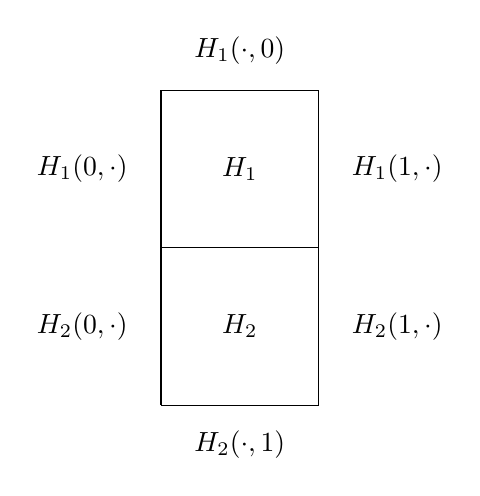
\begin{tikzpicture}[scale=0.5]
  \draw
    (0,0)
    --
    (4,0)
    --
    (4,4)
    --
    (0,4)
    --
    (0,0);
  \draw
    (0,4)
    --
    (0,8)
    --
    (4,8)
    --
    (4,4);
  \draw
    (2,2)
    --
    (2,2) node[fill=white] {$H_{2}$};
  \draw
    (2,6)
    --
    (2,6) node[fill=white] {$H_{1}$};
  \draw
    (2,-1)
    --
    (2,-1) node[fill=white] {$H_{2}(\cdot,1)$};
  \draw
    (2,9)
    --
    (2,9) node[fill=white] {$H_{1}(\cdot,0)$};
  \draw
    (-2,2)
    --
    (-2,2) node[fill=white] {$H_{2}(0,\cdot)$};
  \draw
    (-2,6)
    --
    (-2,6) node[fill=white] {$H_{1}(0,\cdot)$};
  \draw
    (6,2)
    --
    (6,2) node[fill=white] {$H_{2}(1,\cdot)$};
  \draw
    (6,6)
    --
    (6,6) node[fill=white] {$H_{1}(1,\cdot)$};
\end{tikzpicture}
\]
And if the homotopies were $2$-paths from $H_{1}(\cdot,0)$ to $H_{1}(\cdot,1)$ and from $H_{2}(\cdot,0)$ to $H_{2}(\cdot,1)$, respectively, then we would draw
\[
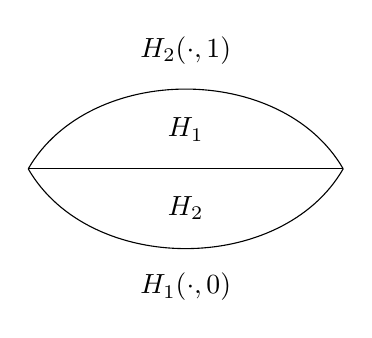
\begin{tikzpicture}[scale=1]
  \draw
    (0,2)
    to[bend left=60]
    (4,2);
  \draw
    (0,2)
    --
    (4,2);
  \draw
    (0,2)
    to[bend right=60]
    (4,2);
  \draw
    (2,2.5)
    --
    (2,2.5) node[fill=white] {$H_{1}$};
  \draw
    (2,1.5)
    --
    (2,1.5) node[fill=white] {$H_{2}$};
  \draw
    (2,0.5)
    --
    (2,0.5) node[fill=white] {$H_{1}(\cdot,0)$};
  \draw
    (2,3.5)
    --
    (2,3.5) node[fill=white] {$H_{2}(\cdot,1)$};
\end{tikzpicture}
\]
And this clearly makes sense for $n > 2$. This composition has the following properties:
\begin{enumerate}
\item[(a)]
It is associative up to homotopy. This is to say that composing $n$-paths is only associative up to an $n+1$-path.
\item[(b)]
Composing an $n$-path with the constant $n$-path (a constant $n$-path is one which is independent of its last coordinate) on the left or on the right reproduces the $n$-path up to homotopy suggesting that the constant $n$-path is an identity up to homotopy. In other words, composing an $n$-path with the constant $n$-path obeys a unital law up to an $n+1$-path.
\item[(c)]
With respect to the identity from (b) one can invert an $n$-path up to homotopy, that is, up to an $n+1$-path.
\end{enumerate}
But this kind of path composition is not the only one for $n \geq 2$. We rather have $n$ compositions for $n$-paths. For if given homotopies
\begin{align*}
  H_{1},H_{2}
  \colon
  I
  \times
  I
  &\rightarrow
  Y
\end{align*}
we can compose homotopies (up to a homotopy of homotopies) along the second coordinate if
\begin{align*}
  H_{1}(1,\cdot)
  &=
  H_{2}(0,\cdot)
\end{align*}
as illustrated by the picture
\[
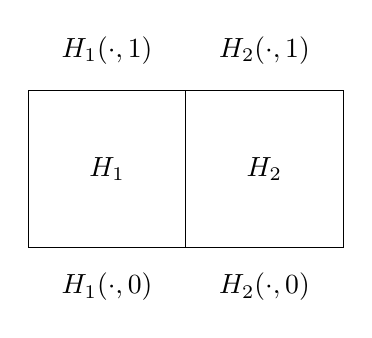
\begin{tikzpicture}[scale=0.5]
  \draw
    (0,0)
    --
    (4,0)
    --
    (4,4)
    --
    (0,4)
    --
    (0,0);
  \draw
    (4,0)
    --
    (8,0)
    --
    (8,4)
    --
    (4,4);
  \draw
    (2,2)
    --
    (2,2) node[fill=white] {$H_{1}$};
  \draw
    (6,2)
    --
    (6,2) node[fill=white] {$H_{2}$};
  \draw
    (2,-1)
    --
    (2,-1) node[fill=white] {$H_{1}(\cdot,0)$};
  \draw
    (6,-1)
    --
    (6,-1) node[fill=white] {$H_{2}(\cdot,0)$};
  \draw
    (2,5)
    --
    (2,5) node[fill=white] {$H_{1}(\cdot,1)$};
  \draw
    (6,5)
    --
    (6,5) node[fill=white] {$H_{2}(\cdot,1)$};
\end{tikzpicture}
\]
And if the homotopies were $2$-paths from $H_{1}(\cdot,0)$ to $H_{1}(\cdot,1)$ and from $H_{2}(\cdot,0)$ to $H_{2}(\cdot,1)$, respectively, then we would draw
\[
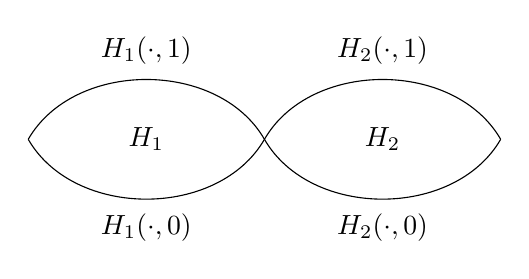
\begin{tikzpicture}[scale=0.75]
  \draw
    (0,2)
    to[bend left=60]
    (4,2);
  \draw
    (0,2)
    to[bend right=60]
    (4,2);
  \draw
    (4,2)
    to[bend left=60]
    (8,2);
  \draw
    (4,2)
    to[bend right=60]
    (8,2);
  \draw
    (2,2)
    --
    (2,2) node[fill=white] {$H_{1}$};
  \draw
    (6,2)
    --
    (6,2) node[fill=white] {$H_{2}$};
  \draw
    (2,0.5)
    --
    (2,0.5) node[fill=white] {$H_{1}(\cdot,0)$};
  \draw
    (6,0.5)
    --
    (6,0.5) node[fill=white] {$H_{2}(\cdot,0)$};
  \draw
    (2,3.5)
    --
    (2,3.5) node[fill=white] {$H_{1}(\cdot,1)$};
  \draw
    (6,3.5)
    --
    (6,3.5) node[fill=white] {$H_{2}(\cdot,1)$};
\end{tikzpicture}
\]
All this also makes sense for $n > 2$. For these compositions we again have associativity, unital laws and invertibility only up to higher paths. But this {\glqq}up to higher paths{\grqq} is not arbitrary in classical homotopy theory. Let us discuss this a bit in the case of composing $1$-paths up to $2$-paths. The point we want to address is that associativity and the identity law of $1$-path composition is up to \underline{coherent} homotopy. This is to say that there is a family $A(p_{1},p_{2},p_{3})$ of homotopies parametrized by appropriate $1$-paths $p_{1},p_{2},p_{3}$ such that given two parenthesizations of a concatenation of arbitrarily many $1$-paths it does not matter (up to homotopy) how we apply the elements of the family $\lbrace A(p_{1},p_{2},p_{3}) \rbrace$ to go from one to the other. This can be derived from the assumption that the $2$-paths
\begin{align*}
  A_{1}
  &:=
  A(p_{2} \circ p_{1},p_{3},p_{4})
  \circ
  A(p_{1},p_{2},p_{4} \circ p_{3})
\end{align*}
and
\begin{align*}
  A_{2}
  &:=
  \left(
    \mathrm{id}_{p_{4}}
    \circ^{\textrm{h}}
    A(p_{1},p_{2},p_{3})
  \right)
  \circ
  A(p_{1},p_{3} \circ p_{2},p_{4})
  \circ
  \left(
    A(p_{2},p_{3},p_{4})
    \circ^{\textrm{h}}
    \mathrm{id}_{p_{1}}
  \right)
\end{align*}
from
\begin{align*}
  \left(
    (p_{4} \circ p_{3})
    \circ
    p_{2}
  \right)
  \circ
  p_{1}
\end{align*}
to
\begin{align*}
  p_{4}
  \circ
  \left(
    p_{3}
    \circ
    (p_{2} \circ p_{1})
  \right)
\end{align*}
are homotopic, that is, the diagram
\[
\begin{tikzcd}[row sep=3.5em,column sep=0.4em]
  &
  (p_{4} \circ p_{3})
  \circ
  (p_{2} \circ p_{1})
  \arrow{dr}{A(p_{2} \circ p_{1},p_{3},p_{4})}
  &
  \\
  \left(
    (p_{4} \circ p_{3})
    \circ
    p_{2}
  \right)
  \circ
  p_{1}
  \arrow{ur}{A(p_{1},p_{2},p_{4} \circ p_{3})}
  \arrow[swap]{d}{A(p_{2},p_{3},p_{4}) \circ^{\textrm{h}} \mathrm{id}_{p_{1}}}
  &
  &
  p_{4}
  \circ
  \left(
    p_{3}
    \circ
    (p_{2} \circ p_{1})
  \right)
  \\
  \left(
    p_{4}
    \circ
    (p_{3} \circ p_{2})
  \right)
  \circ
  p_{1}
  \arrow{rr}{A(p_{1},p_{3} \circ p_{2},p_{4})}
  &
  &
  p_{4}
  \circ
  \left(
    (p_{3} \circ p_{2})
    \circ
    p_{1}
  \right)
  \arrow[swap]{u}{\mathrm{id}_{p_{4}} \circ^{\textrm{h}} A(p_{1},p_{2},p_{3})}
\end{tikzcd}
\]
commutes up to homotopy.
\begin{align*}
  A_{1}
  &\sim
  A_{2}
\end{align*}
is known as Stasheff's pentagon identity. And deriving associativity up to coherent homotopy from Stasheff's pentagon identity can be considered a so-called {\glqq}coherence theorem{\grqq} for the {\glqq}coherence condition{\grqq} $A_{1} \sim A_{2}$. In a similar vein the identity law is treated to obtain a coherence theorem for a coherence condition in this case, too. To this end let $\mathrm{const}_{y}$ denote the $1$-path constant at $y \in Y$. Moreover note that if additionally to the family $A(p_{1},p_{2},p_{3})$ we have for all $1$-paths $p_{1}$ homotopies $R(p_{1})$ from $p_{1} \circ \mathrm{const}_{p_{1}(0)}$ to $p_{1}$ and
$L(p_{1})$ from $\mathrm{const}_{p_{1}(1)} \circ p_{1}$ to $p_{1}$, respectively, then we get that the homotopy
\begin{align*}
  R(p_{2})
  \circ^{\textrm{h}}
  \mathrm{id}_{p_{1}}
\end{align*}
is homotopic to the homotopy
\begin{align*}
  \left(
    \mathrm{id}_{p_{2}}
    \circ^{\textrm{h}}
    L(p_{1})
  \right)
  \circ
  A(p_{1},\mathrm{const}_{p_{1}(1)},p_{2})
\end{align*}
both from
\begin{align*}
  \left(
    p_{2}
    \circ
    \mathrm{const}_{p_{1}(1)}
  \right)
  \circ
  p_{1}
\end{align*}
to
\begin{align*}
  p_{2}
  \circ
  p_{1}
\end{align*}
This means the diagram
\[
\begin{tikzcd}[sep=large]
  \left(
    p_{2}
    \circ
    \mathrm{const}_{p_{1}(1)}
  \right)
  \circ
  p_{1}
  \arrow{rr}{A(p_{1},\mathrm{const}_{p_{1}(1)},p_{2})}
  \arrow[swap]{dr}{R(p_{2}) \circ^{\textrm{h}} \mathrm{id}_{p_{1}}}
  &
  &
  p_{2}
  \circ
  \left(
    \mathrm{const}_{p_{1}(1)}
    \circ
    p_{1}
  \right)
  \arrow{dl}{\mathrm{id}_{p_{2}} \circ^{\textrm{h}} L(p_{1})}
  \\
  &
  p_{2}
  \circ
  p_{1}
  &
\end{tikzcd}
\]
commutes up to homotopy. This is known as triangle identity. And deriving the unit laws up to coherent homotopy from the triangle identity can be considered a so-called {\glqq}coherence theorem{\grqq} for the {\glqq}coherence condition{\grqq} imposed by the triangle identity. In both cases the homotopies making the diagrams {\glqq}commute{\grqq} satisfy their own coherence conditions and so on. \cite{69cbf29c} seems to be a good source to gain insight into this process (after reading these notes).
\item[$\bullet$]
Let $n$ be a natural number and let $(S^{n},s^{n})$ denote a pointed $n$-sphere (as a pointed topological space). Let further $(Y,y)$ denote a pointed space. Then a base-point preserving continuous function $l \colon S^{n} \rightarrow Y$ is called an \textbf{$n$-loop (in $Y$)}. This can be regarded as an $n$-path with starting point and terminus the same point of the space regarded as degenerate $n-1$-path (identity of identity of identity of \ldots). So the same reasoning about composition of $n$-paths applies. But then, by dividing out homotopy from composition of $n$-loops, the $n$-loops for fixed $n$ should form a group. And, indeed,
\begin{align*}
  \pi_{n}(Y,y)
  &:=
  \langle
    S^{n},
    Y
  \rangle
\end{align*}
is called the \textbf{$n$-th homotpy group (of $(Y,y)$)} while the first homotopy group is often called \textbf{fundamental group (of $(Y,y)$)}. For $n \geq 1$, $\pi_{n}$ is actually a functor from $\mathbf{Top}_{\ast}$ to $\mathbf{Grp}$ (and for $n \geq 2$ even to $\mathbf{Ab}$). Note that $\pi_{0}(Y)$ is not actually a group.
\item[$\bullet$]
We can now define categories $\mathbf{HTop}$ and $\mathbf{HTop}_{\ast}$ by
\begin{align*}
  \mathrm{ob}_{\mathbf{HTop}}
  &:=
  \mathrm{ob}_{\mathbf{Top}}
  \\
  \mathrm{mor}_{\mathbf{HTop}}(Y_{1},Y_{2})
  &:=
  [Y_{1},Y_{2}]
\end{align*}
in the unpointed case and
\begin{align*}
  \mathrm{ob}_{\mathbf{HTop}_{\ast}}
  &:=
  \mathrm{ob}_{\mathbf{Top}_{\ast}}
  \\
  \mathrm{mor}_{\mathbf{HTop}_{\ast}}(Y_{1},Y_{2})
  &:=
  \langle
    Y_{1},
    Y_{2}
  \rangle
\end{align*}
in the pointed case. These become categories by noting that we can compose homotopies (relative $A_{1} \subset Y_{1}$) horizontally (up to higher homotopy) as sketched above. $\mathbf{HTop}$ is called \textbf{naive homotopy category (of $\mathbf{Top}$)} while $\mathbf{HTop}_{\ast}$ is called \textbf{(pointed) naive homotopy category (of $\mathbf{Top}_{\ast}$)}. Note that for subcategories $\mathbf{Top}^{\textrm{Name}}$ of $\mathbf{Top}$ and $\mathbf{Top}_{\ast}^{\textrm{Name}}$ of $\mathbf{Top}_{\ast}$ we get according subcategories of the naive homotopy categories which we denote $\mathbf{HTop}^{\textrm{Name}}$ and $\mathbf{HTop}_{\ast}^{\textrm{Name}}$, respectively. $\mathbf{HTop}^{\textrm{Name}}$ is called \textbf{naive homotopy category (of $\mathbf{Top}^{\mathrm{Name}}$)} while $\mathbf{HTop}_{\ast}^{\textrm{Name}}$ is called \textbf{(pointed) naive homotopy category (of $\mathbf{Top}_{\ast}^{\mathrm{Name}}$)}. The functors $\pi_{n}$ can now be made into functors on $\mathbf{HTop}_{\ast}$.
\item[$\bullet$]
Representatives of isomorphisms of $\mathbf{HTop}$ are called \textbf{strong homotopy equivalences}. Assume a strong homotopy equivalence $f \colon Y_{1} \rightarrow Y_{2}$. Then due to theorem \ref{thm:catiso} we have that
\begin{align*}
  \pi_{n}([f])
  &=
  \pi_{n}(f)
\end{align*}
is an isomorphism. This gives rise to an idea of a weaker notion of homotopy equivalence. At this point note that {\glqq}strong{\grqq} is not really standard in traditional literature. But we will explain in a moment why we opted for it. A morphism $f \colon Y_{1} \rightarrow Y_{2}$ of $\mathbf{Top}$ or $\mathbf{Top}_{\ast}$ is called \textbf{(weak) homotopy equivalence (of $Y_{1}$ and $Y_{2}$)} if $\pi_{n}(f)$ is an isomorphism for all $n \in \mathbb{N}$. Homotopy equivalences are not strong homotopy equivalences in general but they are for CW complexes. The latter fact is known as Whitehead's theorem.
\item[$\bullet$]
If there is an $n_{0} \in \mathbb{N}$ such that for all $n > n_{0}$ the homotopy groups $\pi_{n}(Y,y)$ consist of a single element we say that $Y$ is a \textbf {(topological) homotopy $n_{0}$-type}, else we say that $Y$ is a \textbf{(topological) homotopy $\infty$-type}. Note that this is not always standard terminology. We discuss this in a moment.
\end{enumerate}
This review of classical homotopy theory has a few implications which are the topic of the rest of this subsection.
\\
We paid attention chiefly to $n$-paths. You might guess why: the $1$-paths in a topological space $Y$ behave as the morphisms in a groupoid if we factor out homotopies. Formally, for a topological space $Y$ define a groupoid $\Pi_{1}(Y)$ with objects just the points of the space $Y$ and morphisms from a point $y_{1}$ to a point $y_{2}$ of $Y$ just the homotopy classes of paths from $y_{1}$ to $y_{2}$ by the (C3) trick from remark \ref{rem:c3trick}. Clearly the morphisms from $y \in Y$ to itself are the same as the group $\pi_{1}(Y,y) = \langle S^{1},Y \rangle$. $\Pi_{1}(Y)$ is the literally fundamental example of groupoids and is therefore called \textbf{fundamental groupoid (of $Y$)}. But we can see even more. Namely, $2$-paths behave just as we wished the $2$-morphisms of a weak $2$-groupoid to behave. But we now have a real idea for conditions when the notion of associativity and unit law is {\glqq}coherent{\grqq}: We weaken as proposed before the classical homotopy theory discussion but motivated from classical homotopy theory we also demand
\begin{enumerate}
\item[(1)]
\begin{align*}
  \mathsf{A}_{1}
  &=
  \mathsf{A}_{2}
\end{align*}
\item[(2)]
\begin{align*}
  \mathsf{R}(f_{23})
  \circ^{\textrm{h}}
  \mathrm{id}_{f_{12}}
  &=
  \left(
    \mathrm{id}_{f_{23}}
    \circ^{\textrm{h}}
    \mathsf{L}(f_{12})
  \right)
  \circ
  \mathsf{A}(f_{12},\mathsf{id}_{X_{2}},f_{23})
\end{align*}
\end{enumerate}
If one can then prove an appropriate coherence theorem to interpret these as coherence conditions - and one can as Mac Lane has shown - then we are done. So let us formally define weak $2$-category\footnote{for historical reasons this is sometimes called bicategory}. A set ${}_{2}\mathbf{C}$ is a \textbf{(weak) $2$-category} if it is a $3$-tuple consisting of a set ${}_{0}\mathrm{mor}_{{}_{2}\mathbf{C}}$, for all $X_{1},X_{2} \in {}_{0}\mathrm{mor}_{_{2}\mathbf{C}}$ a category
\begin{align*}
  \left(
    {}_{1}\mathrm{mor}_{{}_{2}\mathbf{C}}(X_{1},X_{2}),
    {}_{2}\mathrm{mor}_{{}_{2}\mathbf{C}}(X_{1},X_{2},\cdot,\cdot),
    \circ_{(X_{1},X_{2})}^{\textrm{v}}
  \right)
  &:=
  {}_{1}\mathbf{mor}_{{}_{2}\mathbf{C}}(X_{1},X_{2})
\end{align*}
and for all $X_{1},X_{2},X_{3} \in {}_{0}\mathrm{mor}_{{}_{2}\mathbf{C}}$ a functor\footnote{if you really want to understand this you have to jump to subsection \ref{sec:prodcat} about product categories right at the beginning but you can also ignore it because it is not really the point for what follows beyond this definition}
\begin{align*}
  \circ^{\textrm{h}}
  \doteq
  \circ^{\textrm{h}}(X_{1},X_{2},X_{3})
  \doteq
  \circ_{{}_{2}{\mathbf{C}}}^{\textrm{h}}(X_{1},X_{2},X_{3})
  \colon
  {}_{1}\mathbf{mor}_{{}_{2}\mathbf{C}}(X_{1},X_{2})
  \times
  {}_{1}\mathbf{mor}_{{}_{2}\mathbf{C}}(X_{2},X_{3})
  &\rightarrow
  {}_{1}\mathbf{mor}_{{}_{2}\mathbf{C}}(X_{1},X_{3})
\end{align*}
such that
\begin{enumerate}
\item[(${}_{2}$C0)]
The $3$-tuple\footnote{note that a functor is a $4$-tuple and projection to the third coordinate is the object part}
\begin{align*}
  \left(
    {}_{0}\mathrm{mor}_{{}_{2}\mathbf{C}},
    {}_{1}\mathrm{mor}_{{}_{2}\mathbf{C}},
    \circ_{\mathbf{C}}
  \right)
\end{align*}
with
\begin{align*}
  \circ_{\mathbf{C}}
  &:=
  \circ^{1}
  \left(
    \circ_{{}_{2}\mathbf{C}}^{\textrm{h}},
    \mathrm{pr}_{3}
  \right)
\end{align*}
is such that
\begin{enumerate}
\item[(WC1)]
for all $X_{1},X_{2},X_{3},X_{4}$ there is a natural isomorphism
\begin{align*}
  \mathsf{A}
  &\doteq
  \mathsf{A}
  \left(
    X_{1},
    X_{2},
    X_{3},
    X_{4}
  \right)
\end{align*}
from
\begin{align*}
  \left(
    \cdot
    \circ
    \cdot
  \right)
  \circ
  \cdot
  &\doteq
  \circ^{\textrm{h}}(X_{1},X_{2},X_{4})
  \left(
    \cdot,
    \circ^{\textrm{h}}
    (X_{2},X_{3},X_{4})
    (\cdot,\cdot)
  \right)
\end{align*}
to
\begin{align*}
  \cdot
  \circ
  \left(
    \cdot
    \circ
    \cdot
  \right)
  &\doteq
  \circ^{\textrm{h}}
  (X_{1},X_{3},X_{4})
  \left(
    \circ^{\textrm{h}}
    (X_{1},X_{2},X_{3})
    (\cdot,\cdot),
    \cdot
  \right)
\end{align*}
making for all $f_{12},f_{23},f_{34},f_{45}$ the diagram
\[
\begin{tikzcd}[row sep=3.5em,column sep=0.4em]
  &
  (f_{45} \circ f_{34})
  \circ
  (f_{23} \circ f_{12})
  \arrow{dr}{\mathsf{A}(f_{23} \circ f_{12},f_{34},f_{45})}
  &
  \\
  \left(
    (f_{45} \circ f_{34})
    \circ
    f_{23}
  \right)
  \circ
  f_{12}
  \arrow{ur}{\mathsf{A}(f_{12},f_{23},f_{45} \circ f_{34})}
  \arrow[swap]{d}{\mathsf{A}(f_{23},f_{34},f_{45}) \circ^{\textrm{h}} \mathrm{id}_{f_{12}}}
  &
  &
  f_{45}
  \circ
  \left(
    f_{34}
    \circ
    (f_{23} \circ f_{12})
  \right)
  \\
  \left(
    f_{45}
    \circ
    (f_{34} \circ f_{23})
  \right)
  \circ
  f_{12}
  \arrow{rr}{\mathsf{A}(f_{12},f_{34} \circ f_{23},f_{45})}
  &
  &
  f_{45}
  \circ
  \left(
    (f_{34} \circ f_{23})
    \circ
    f_{12}
  \right)
  \arrow[swap]{u}{\mathrm{id}_{f_{45}} \circ^{\textrm{h}} \mathsf{A}(f_{12},f_{23},f_{34})}
\end{tikzcd}
\]
commute
\item[(WC2)]
for each $X_{1} \in \mathrm{ob}_{\mathbf{C}}$ there is an element
\begin{align*}
  \mathrm{id}_{X_{1}}
  &\in
  \mathrm{mor}_{\mathbf{C}}(X_{1},X_{1})
\end{align*}
and natural isomorphisms
\begin{align*}
  \mathsf{R}
  \doteq
  \mathsf{R}(X_{1})
  \colon
  \circ^{\textrm{h}}(\mathrm{id}_{X_{1}},\cdot)
  &\Rightarrow
  \mathrm{id}_{{}_{1}\mathbf{mor}_{{}_{2}}\mathbf{C}(X_{1},X_{2})}
  \\
  \mathsf{L}
  \doteq
  \mathsf{L}(X_{1})
  \colon
  \circ^{\textrm{h}}(\cdot,\mathrm{id}_{X_{2}})
  &\Rightarrow
  \mathrm{id}_{{}_{1}\mathbf{mor}_{{}_{2}}\mathbf{C}(X_{1},X_{2})}
\end{align*}
making for all $f_{12},f_{23}$ the diagram
\[
\begin{tikzcd}[sep=large]
  \left(
    f_{23}
    \circ
    \mathrm{id}_{X_{2}}
  \right)
  \circ
  f_{12}
  \arrow{rr}{\mathsf{A}(f_{12},\mathrm{id}_{X_{2}},f_{23})}
  \arrow[swap]{dr}{\mathsf{R}(f_{23}) \circ^{\textrm{h}} \mathrm{id}_{f_{12}}}
  &
  &
  f_{23}
  \circ
  \left(
    \mathrm{id}_{X_{2}}
    \circ
    f_{12}
  \right)
  \arrow{dl}{\mathrm{id}_{f_{23}} \circ^{\textrm{h}} \mathsf{L}(f_{12})}
  \\
  &
  f_{23}
  \circ
  f_{12}
  &
\end{tikzcd}
\]
commute
\item[(WC3)]
for all
\begin{align*}
  (X_{1},X_{2}),(X_{3},X_{4})
  &\in
  \mathrm{ob}_{\mathbf{C}}
  \times
  \mathrm{ob}_{\mathbf{C}}
\end{align*}
satisfying
\begin{align*}
  (X_{1},X_{2})
  &\neq
  (X_{3},X_{4})
\end{align*}
the the formula
\begin{align*}
  \mathrm{mor}_{\mathbf{C}}(X_{1},X_{2})
  \cap
  \mathrm{mor}_{\mathbf{C}}(X_{3},X_{4})
  &=
  \emptyset
\end{align*}
holds\footnote{this last property is a peculiarity of materlial set theories such as TG if we want the category definition to be exactly the same as the usual first order theory of category theory}.
\end{enumerate}
\item[(${}_{2}$C1)]
for all $X_{1},X_{2},X_{3},X_{4} \in {}_{0}\mathrm{mor}_{{}_{2}\mathbf{C}}$, for all
\begin{align*}
  f_{12},f_{12}^{\backprime}
  &\in
  {}_{1}\mathrm{mor}_{{}_{2}\mathbf{C}}(X_{1},X_{2})
  \\
  f_{23},f_{23}^{\backprime}
  &\in
  {}_{1}\mathrm{mor}_{{}_{2}\mathbf{C}}(X_{2},X_{3})
  \\
  f_{34},f_{34}^{\backprime}
  &\in
  {}_{1}\mathrm{mor}_{{}_{2}\mathbf{C}}(X_{3},X_{4})
\end{align*}
and for all
\begin{align*}
  {}_{2}f_{\alpha}
  &\in
  {}_{2}\mathrm{mor}_{{}_{2}\mathbf{C}}(X_{1},X_{2},f_{12},f_{12}^{\backprime})
  \\
  {}_{2}f_{\beta}
  &\in
  {}_{2}\mathrm{mor}_{{}_{2}\mathbf{C}}(X_{2},X_{3},f_{23},f_{23}^{\backprime})
  \\
  {}_{2}f_{\gamma}
  &\in
  {}_{2}\mathrm{mor}_{{}_{2}\mathbf{C}}(X_{3},X_{4},f_{34},f_{34}^{\backprime})
\end{align*}
the term
\begin{align*}
  \circ_{{}_{2}\mathbf{C}}^{\textrm{h}}
  (X_{1},X_{2},X_{4})
  \left(
    {}_{2}f_{\alpha},
    \circ_{{}_{2}\mathbf{C}}^{\textrm{h}}
    (X_{2},X_{3},X_{4})
    ({}_{2}f_{\beta},{}_{2}f_{\gamma})
  \right)
\end{align*}
equals the term
\begin{align*}
  \circ_{{}_{2}\mathbf{C}}^{\textrm{h}}
  (X_{1},X_{3},X_{4})
  \left(
    \circ_{{}_{2}\mathbf{C}}^{\textrm{h}}
    (X_{1},X_{2},X_{3})
    ({}_{2}f_{\alpha},{}_{2}f_{\beta}),
    {}_{2}f_{\gamma}
  \right)
\end{align*}
\item[(${}_{2}$C2)]
for each $X_{1} \in {}_{0}\mathrm{mor}_{{}_{2}\mathbf{C}}$ the identity $\mathrm{id}_{\mathrm{id}_{X_{1}}}$ of the identity $\mathrm{id}_{X_{1}}$ of $X_{1}$ (the former w.r.t. ${}_{1}\mathbf{mor}_{{}_{2}\mathbf{C}}(X_{1},X_{2})$, the latter w.r.t. the category from property (${}_{2}$C0)) satisfies for all
\begin{align*}
  f_{12},f_{12}^{\backprime}
  &\in
  {}_{1}\mathrm{mor}_{{}_{2}\mathbf{C}}(X_{1},X_{2})
  \\
  f_{21},f_{21}^{\backprime}
  &\in
  {}_{1}\mathrm{mor}_{{}_{2}\mathbf{C}}(X_{2},X_{1})
\end{align*}
and for all
\begin{align*}
  {}_{2}f_{\alpha}
  &\in
  {}_{2}\mathrm{mor}_{{}_{2}\mathbf{C}}(X_{1},X_{2},f_{12},f_{12}^{\backprime})
  \\
  {}_{2}f_{\beta}
  &\in
  {}_{2}\mathrm{mor}_{{}_{2}\mathbf{C}}(X_{2},X_{1},f_{21},f_{21}^{\backprime})
\end{align*}
with $X_{2} \in {}_{0}\mathrm{mor}_{{}_{2}\mathbf{C}}$ both
\begin{align*}
  \circ_{{}_{2}\mathbf{C}}^{\textrm{h}}
  (X_{1},X_{1},X_{2})
  (\mathrm{id}_{\mathrm{id}_{X_{1}}},{}_{2}f_{\alpha})
  &=
  {}_{2}f_{\alpha}
\end{align*}
and
\begin{align*}
  \circ_{{}_{2}\mathbf{C}}^{\textrm{h}}
  (X_{2},X_{1},X_{1})
  ({}_{2}f_{\beta},\mathrm{id}_{\mathrm{id}_{X_{1}}})
  &=
  {}_{2}f_{\beta}
\end{align*}
\item[(${}_{2}$C3)]
for all $X_{1},X_{2},X_{3},X_{4} \in {}_{0}\mathrm{mor}_{{}_{2}\mathbf{C}}$, for all
\begin{align*}
  f_{12},f_{12}^{\backprime}
  &\in
  {}_{1}\mathrm{mor}_{{}_{2}\mathbf{C}}(X_{1},X_{2})
  \\
  f_{34},f_{34}^{\backprime}
  &\in
  {}_{1}\mathrm{mor}_{{}_{2}\mathbf{C}}(X_{3},X_{4})
\end{align*}
such that
\begin{align*}
  (X_{1},X_{2},f_{12},f_{12}^{\backprime})
  &\neq
  (X_{3},X_{4},f_{34},f_{34}^{\backprime})
\end{align*}
the formula
\begin{align*}
  {}_{2}\mathrm{mor}_{{}_{2}\mathbf{C}}(X_{1},X_{2}f_{12},f_{12}^{\backprime})
  \cap
  {}_{2}\mathrm{mor}_{{}_{2}\mathbf{C}}(X_{3},X_{4}f_{34},f_{34}^{\backprime})
  &=
  \emptyset
\end{align*}
holds\footnote{this property is again an annoying technicality of material set theories}
\end{enumerate}
You see right. Only property (${}_{2}$C0) differs from the definition of a strict category in that we do not demand category anymore but only category with associativity and unit law up to coherent isomorphism. This way can be gone further to obtain even higher categories since we have taken only homotopy up to dimension $2$ into account yet. This is a really artificial restriction and we should actually take all $n$-paths into account to obtain the fundamental $\infty$-groupoid of a space $Y$ as an informal weak $\infty$-groupoid. Then in a similar manner we can try to get ideas for coherence conditions to yield a definition of weak higher categories (and hence groupoids) if we can show the coherence theorems for these coherence conditions. However, this is still a terribly complicated process and once more homotopy theory may help by the following observation. Having the definition of weak $2$-groupoids as above then if $Y$ is a
\begin{enumerate}
\item[(0)]
topological homotopy $0$-type, the fundamental $2$-groupoid of $Y$ has as $1$-morphisms only identity $1$-morphisms (up to coherent homotopy) and as $2$-morphisms only identity $2$-morphisms. Hence it is actually just a set of $0$-morphisms - a set, a discrete $2$-groupoid or say $0$-groupoid. And of course, any $0$-groupoid can be regarded as fundamental $2$-groupoid for some topological homotopy $0$-type.
\item[(1)]
topological homotopy $1$-type, the fundamental $2$-groupoid of $Y$ has as $2$-morphisms only identity $2$-morphisms. Hence it is actually just a common groupoid. And of course, any $1$-groupoid can be regarded as fundamental groupoid for some topological homotopy $1$-type.
\item[(2)]
topological homotopy $2$-type, the fundamental $2$-groupoid $Y$ is some $2$-groupoid. And of course, any $2$-groupoid can be regarded as fundamental $2$-groupoid for some topological homotopy $2$-type.
\end{enumerate}
Hence the topological spaces up to weak homotopy equivalence correspond to weak $2$-groupoids. Is this generalizable to higher dimensions? This is what Grothendieck famously conjectured: The Grothendieck hypothesis.
\\
\begin{prp}[Grothendieck]
\label{prp:groth}
(Weak) $n$-groupoids are equivalent to topological homotopy $n$-types for $n \in \mathbb{N} \cup \lbrace \infty \rbrace$.
\end{prp}
\begin{prf}
That depends a bit as we will now see.
\\
\phantom{proven}
\hfill
$\square$
\end{prf}
The truth of the Grothendieck hypothesis \ref{prp:groth} depends on the definition of higher groupoids. If we define groupoids as suggested then it is trivially true. However, proceeding from this definition of higher groupoids makes it hard to define higher categories since we have to prove coherence theorems for all the coherence conditions in all dimensions to show this definition of higher categories to be sensible. On the other hand it is quite easy to get higher groupoids from higher categories. This suggests to use the Grothendieck hypothesis \ref{prp:groth} indirectly as consistency test for a definition of higher categories to check that the definition is coherent in the sense that even if the coherence conditions do not appear in the higher category definition - and that is what we actually want - they are still present. This is to say that the Grothendieck hypothesis \ref{prp:groth} as theorem is a litmus test for a sensible definition of higher categories with weak associatively composable higher directed paths obeying a weak identity law. This is how higher category theory is done nowadays. We will provide some literature on the topic in section \ref{sec:metaidea} where we elaborate on it a bit further.
\\
A further implication of the review of classical homotopy theory is the impression that homotopy theory is more about paths than homotopies between functions. Of course, you can object now that, by definition, paths are actually homotopies in classical homotopy theory. But note that we could fully capture the behavior of the $n$-paths we have in mind by $\infty$-groupoids when we demand the Grothendieck hypothesis \ref{prp:groth}. The $n$-paths are then {\glqq}synthetic{\grqq} and hence have a built-in continuity (contrary to the model of paths as certain continuous\footnote{in the sense of topology} functions). The {\glqq}continuity{\grqq} is then trivially the intuitively correct one for paths which are characterized by higher groupoid theory (not interpreted in a set theory but rather as formal theory). This is in analogy to how the elements of a set are trivially what we want elements of a collection to be. So we cannot get problems regarding continuity as in topology described in example \ref{exa:topology} (where the problems might be inherited from those of the notion of nearness). Moreover note that homotopies in classical homotopy theory actually behave in the same way as paths in an $\infty$-groupoid:
\begin{enumerate}
\item[(1)]
they can be composed associatively up to coherent homotopy
\item[(2)]
there is an identity law for a constant homotopy up to coherent homotopy
\item[(3)]
homotopies are invertible up to coherent homotopy
\end{enumerate}
Additionally, homotopy between functions is by the very idea a way to go from a function to another without really changing its continuity structure. It is essentially still the same function w.r.t. to continuity. Further, being homotopic as equivalence relation further emphasizes that being homotopic is the structural equality of continuous functions. In other words, homotopy is isomorphism for contiuous functions. This is perfectly reflected by the categories $\mathbf{HTop}$ and $\mathbf{HTop}_{\ast}$, respectively. And so we cannot help to think of homotopies as $1$-paths in a groupoid with objects some continuous functions. We can even sort of see the path aspect of homotopies in classical homotopy theory. To this end note that a homotopy $H$ from $f$ to $f^{\backprime}$ defines functions
\begin{align*}
  p_{H}
  \colon
  I
  &\rightarrow
  \mathrm{mor}_{\mathbf{Top}}(Y_{1},Y_{2})
  \\
  t
  &\mapsto
  H(\cdot,t)
  \\
  h
  \colon
  Y_{1}
  &\rightarrow
  \mathrm{mor}_{\mathbf{Top}}(I,Y_{2})
  \\
  y_{1}
  &\mapsto
  H(y_{1},\cdot)
\end{align*}
So $p_{H}$ suggests to consider a homotopy as a path in $\mathrm{mor}_{\mathbf{Top}}(Y_{1},Y_{2})$ while $h$ suggests to consider it a family of paths in $Y_{2}$ indexed by $Y_{1}$. Both ideas have the problem that it is not clear how to reasonably topologize $\mathrm{mor}_{\mathbf{Top}}(Y_{1},Y_{2})$ and $\mathrm{mor}_{\mathbf{Top}}(I,Y_{2})$ to make both $p_{H}$ and $h$ equivalent to $H$. This is to say that it is not clear how to define when two continuous functions are near each other. This is a common problem in different fields of mathematics. Anyways, it should intuitively hold that $p_{H}$ and $h$ are equivalent to $H$. This is even desirable in classical homotopy theory since there are some inconveniences\footnote{e.g. w.r.t. fiber and cofiber sequences} if it does not hold. This is why one usually restricts to a convenient category of topological spaces for the purpose of classical homotopy theory. We will say what that means in subsection \ref{sec:adjoint}. Anyways, what this tells us about classical homotopy theory is that it is more about $n$-paths than homotopies between continuous functions. This may seem odd to you if you are used to traditional books on algebraic topology and you might object that it is somewhat arbitrary to require homotopies to be equivalent to $p_{H}$ and $h$. But note that the only thing that fails in general is continuity in the sense of topology as described in example \ref{exa:topology}. But there we argued that continuity in that sense does not perfectly match the human idea of continuity. But for the purpose of paths we are interested in an intuitive continuity of these and hence $\mathbf{Top}$ cannot be the ideal setting. Though it is known to be a good approximation of the intuitive idea - at least when restricted to spaces with good separation properties. In this context it is interesting that the objects of the usual convenient category\footnote{so-called compactly generated spaces} are at least Fr\'{e}chet spaces, that is, fulfill the separation axiom $T_{1}$. Now the homotopy as path (or say structural equality) thinking has a consequence for what we consider a topological homotopy type. Our definition of those is in contrast to the original idea that topological spaces have the same homotopy type if and only if they are strongly homotopy equivalent. But in the light of higher category theory this is too strong. Just look at $\mathbf{Top}$. $f \colon Y_{1} \rightarrow Y_{2}$ is an isomorphism in $\mathbf{Top}$ if there is a morphism $f^{-1} \colon Y_{2} \rightarrow Y_{1}$ in $\mathbf{Top}$ such that
\begin{align*}
  f^{-1}
  \circ
  f
  &=
  \mathrm{id}_{Y_{1}}
  \\
  f
  \circ
  f^{-1}
  &=
  \mathrm{id}_{Y_{2}}
\end{align*}
A strong homotopy equivalence is then just weakening these equations to homotopies. This is to say that strong homotopy equivalence is isomorphism in $\mathbf{Top}$ (hypothetically) regarded as weak $2$-category with $2$-morphisms the homotopies (and hence all $2$-morphisms invertible). But why should we not take homotopies between homotopies into account and weaken to a $3$-categorical setting (if we have one)? This would be like stop counting at some arbitrarily chosen number. While this seems a philosophically legit stance\footnote{ultrafinitism} this thinking is rejected by most mathematicians. So if one does not explicitly want to examine topological spaces as the things they are but rather wants to examine their homotopy in our $n$-path sense with a notion of continuity as intuitive as possible then the homotopy types defined here are what one is interested in. In particular, if you are interested in physics our notion of homotopy types seems to matter more in the light of \cite{a565d200}. There, to model spacetime one uses homotopy types which are smooth in a precise sense instead of the usual manifolds which rest at topological spaces to capture nearness. \cite{a565d200} seems kind of successful to us and the purpose of these notes is among other things a soft first step to understand what is done there. But now back to the notion equality. The above motivates some more thoughts about {\glqq}being same{\grqq} in $\mathbf{Cat}$. Two objects $X_{1}$ and $X_{2}$ of a $2$-category are considered the same if they are isomorphic up to coherent isomorphism, that is, if there is a $1$-morphism from $X_{1}$ to $X_{2}$ which is reversible up to isomorphism. Written down formally this looks like the formula of strong homotopy equivalence of spaces $Y_{1}$ and $Y_{2}$. Though $\mathbf{Cat}$ is considered a strict $2$-category it makes sense to define a weaker notion of being the same than isomorphism, motivated from the weak $2$-category case. So $F_{\alpha\beta}$ is an \textbf{equivalence (from $\mathbf{C}_{\alpha}$ to $\mathbf{C}_{\beta}$)} if there is $F_{\beta\alpha}$ such that there exist natural isomorphisms from $F_{\beta\alpha} \circ F_{\alpha\beta}$ to $\mathrm{id}_{\mathbf{C}_{\alpha}}$ and from $F_{\alpha\beta} \circ F_{\beta\alpha}$ to $\mathrm{id}_{\mathbf{C}_{\beta}}$. $F_{\beta\alpha}$ is then called \textbf{weak inverse (of $F_{\alpha\beta}$)}. Moreover if $F_{\alpha\beta}$ is an equivalence from $\mathbf{C}_{\alpha}$ to $\mathbf{C}_{\beta}$ we say $\mathbf{C}_{\alpha},\mathbf{C}_{\beta}$ are \textbf{equivalent} and write
\begin{align*}
  \mathbf{C}_{\alpha}
  &\simeq
  \mathbf{C}_{\beta}
\end{align*}
Many properties of categories are still invariant under this weaker notion of being the same. We just have to follow the {\glqq}principle of equivalence{\grqq}. Informally, this means that we should compare objects of a category always just for isomorphism and not for equality. Or more general, equality is only appropriate for the highest morphism level whereas on the other levels we should use coherent isomorphisms. Formally, we can express this in UFP-HoTT using the already adressed univalence axiom. The basic mathematical objects of UFP-HoTT are $\infty$-groupoids. Let us roughly explain how this works. The things in the mathematical universe are types and types can have inhabitants. For $x$ inhabiting the type $X$ one usually writes $x \colon X$. There are types with inhabitants types and any type inhabits such a type. So these types are in spirit as the Grothendieck universes here. To assure the $\infty$-groupoid behavior of the types one demands that for any type $X$ and inhabitants $x_{1}$ and $x_{2}$ of $X$ there is a type $x_{1} =_{X} x_{2}$ and we have an inhabitant $\mathrm{refl}_{x} \colon x =_{X} x$ for all $x \colon X$. This can be understood as the type of paths from $x_{1}$ to $x_{2}$ (or proofs of equality of $x_{1}$ and $x_{2}$ if you like) and an identity path from $x = x$ where $\mathrm{refl}_{x}$ shall stand for reflexivity. Since the so called identity type $x_{1} =_{X} x_{2}$ is itself a type we can repeat this to get ($2$-)paths and so on. This is the essence of the $n$-path definition in classical homotopy theory. These identity types are governed by a universal property\footnote{in the sense we introduce in section \ref{sec:uni}} which is called path induction. It means that if we have a type $C(x_{1},x_{2},p)$ for each path $p \colon x_{1} =_{X} x_{2}$ in a type $X$ then suffices to show that all the $C(x,x,\mathrm{refl}_{x})$ are inhabited to conclude that all $C(x_{1},x_{2},p)$ are inhabited. This can be interpreted classically as a characterization of the free path space. This induction is in analogy to the one of natural numbers where it suffices to proof a property depending on a natural number to be true for $0$ and if it is true for some $n$ then also for $n+1$ to conlude that it is true for all natural numbers. One then wants all (higher\footnote{here also higher paths and not only inhabitants play a role}) inductive types to exist. This includes product types, sum types and function types\footnote{think about the notation $f \colon X_{1} \rightarrow X_{2}$ at this point} for example. Then univalence, which is roughly the statement that
\begin{enumerate}
\item[$\bullet$]
two inhabitants $X_{1},X_{2}$ of a universe $\mathcal{U}$ are equal in the sense $X_{1} =_{\mathcal{U}} X_{2}$ if and only if $X_{1}$ is equivalent to $X_{2}$ which means there is a function\footnote{this is actually an $\infty$-functor} from $X_{1}$ to $X_{2}$ with left and right inverse.
\end{enumerate}
assures the homotopy behaviour and the Grothendieck hypothesis \ref{prp:groth} is true. This is what makes UFP-HoTT a synthetic homotopy theory\footnote{this is to classical homotopy theory as Euclidean geometry is to analytic geometry if classical homotopy theory is understood in the homotopy type sense} and at the same time a very interesting possible foundation of mathematics since it is clear that sets are only a special case of $\infty$-groupoids - or better in this context: homotopy types. We do not want to do UFP-HoTT here too much but we will often allude to it in these notes. If you are interested in homotopy theory (as a reader interested in physics should be) then you should definitely read the really amazing HoTT book \cite{1ba1603e}. Now back to the principle of equivalence we promised being formalizable in the UFP-HoTT: Assume an $\infty$-groupoid/(homotopy) type $X$ and a property $P$ depending on objects/inhabitants/points of $X$ - this is informally\footnote{formally it would be a function from $X$ to a universe of types} a statement depending on the inhabitants of $X$ - then $P$ is called \textbf{compatible with equivalence} if for inhabitants $x_{1}$ and $x_{2}$ connected by a path of $X$ we have the statement: $P(x_{1})$ is true if and only if $P(x_{2})$ is true. Anyways this should make clear why we defined embedding as fully faithful functor. We want to adhere to the principle of equivalence which prevents us from demanding injectivity on objects but rather suggests to take injectivity up to isomorphism on objects what we automatically get from theorem \ref{thm:catiso} for embeddings. There is still another good reason to define embedding as we did. It is derived from embeddings of topological spaces and the relation of topological spaces to the {\glqq}topos of sheaves on a space{\grqq}. But we have to work a bit until we can define this at all. Overall, we recommend to read the rest of the notes before diving into higher category theory and homotopy theory where required since we develop many ideas one needs there.
\\
Last let us emphasize that homotopy theory in our $\infty$-groupoid sense is a special case of higher category theory which was already recognized by Grothendieck. We will seize that idea again in section \ref{sec:metaidea}.
